\documentclass{beamer}

\usepackage{tikz}
\usetikzlibrary{tikzmark,er}
\usepackage{xcolor}

\mode<presentation>{
	\usetheme{Madrid}
	\usecolortheme{whale}
	\setbeamercovered{transparent}
}

\title[CIMIS]{{\small CS293S: Internet of Things}\\An In-Depth Analysis on Weather Data from CIMIS: Estimating Evapotranspiration (ET) Values}
\author[TheShambles]{Nazmus Saquib \and Udit Paul \and Alex Ermakov \and Santha Ramamoorthy}
\institute[CS grads, UCSB]{Graduate Students\\
Department of Computer Science\\
University of California Santa Barbara}
\titlegraphic{
\includegraphics[width=0.2\textwidth]{ucsb-logo.png}}

\AtBeginSection[]
{
  \begin{frame}<beamer>
    \frametitle{Outline}
    \tableofcontents[currentsection]
  \end{frame}
}

\begin{document}
\newcommand{\continued}{\textit{(Cntd.)}}
\newcommand{\tikzstatement}[1]{\tikz\node[draw, align=center,minimum width=12cm,minimum height=1cm,fill=blue!20, text width=12cm]{#1};}
\newcommand{\tikzproblem}[1]{\tikz\node[draw, align=center,minimum width=12cm,minimum height=1cm,fill=red!20, text width=12cm]{#1};}
\newcommand{\tikzsolution}[1]{\tikz\node[draw, align=center,minimum width=12cm,minimum height=1cm,fill=green!20, text width=12cm]{#1};}
%titlepage
\begin{frame}
\titlepage
\end{frame}

\begin{frame}
	\frametitle{Outline}
	\tableofcontents
\end{frame}

\section{Introduction}
\begin{frame}
\frametitle{Introduction: Evapotranspiration (ET)}
\begin{columns}
	\begin{column}{0.5\textwidth}
		\begin{itemize}
		\setlength\itemsep{1em}
		\item Loss of water through:\\
			\begin{enumerate}
				\setlength\itemsep{1em}
				\item Evaporation and 
				\item Transpiration
			\end{enumerate}
		\item Applications:\\
			\begin{itemize}
				\setlength\itemsep{1em}
				\item Irrigation scheduling
				\item Water resource planning, etc.
			\end{itemize}
		\end{itemize}
	\end{column}
	\begin{column}{0.5\textwidth}
		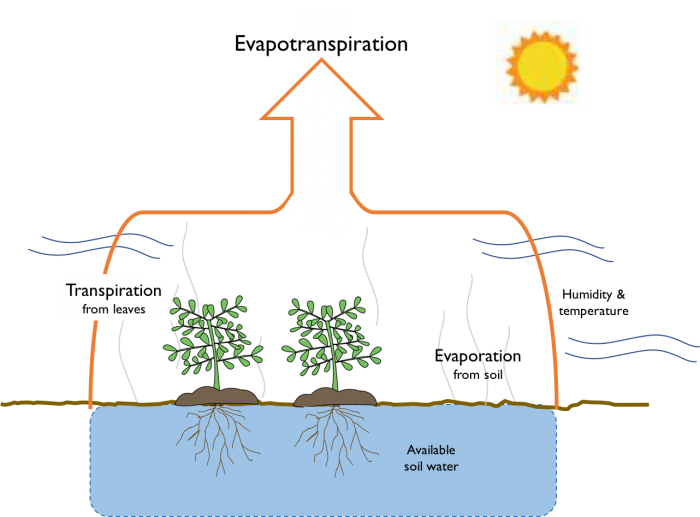
\includegraphics[width=\textwidth]{images/evapotranspiration.png}
	\end{column}
\end{columns}
\end{frame}

\begin{frame}
\frametitle{Introduction: CIMIS Weather Stations}
\begin{itemize}
\setlength\itemsep{1em}
\item \textit{California Irrigation Management Information System}
\item 257 CIMIS stations all through California\\
	\begin{itemize}
		\item 136 actively reports ET values
	\end{itemize}
\item Measures various weather parameters
\item some directly influence ET
\item Also measures (\textit{calculates?}) ET 
\end{itemize}
\end{frame}

\section{Data Collection}
\begin{frame}
\frametitle{Data Collection}
\begin{itemize}
\setlength\itemsep{1em}
\item Publicly available API
\item Reports both hourly and daily data
\item A record contains 16 different features
\item Current working dataset: data of last one year
\item Working dataset will be extended to multiple years:\\
	\begin{itemize}
	\item better for capturing seasonal variations
	\end{itemize}
\end{itemize}
\end{frame}

\section{Data Overview}
\begin{frame}
\frametitle{Sample Hourly ET Values}
\begin{figure}
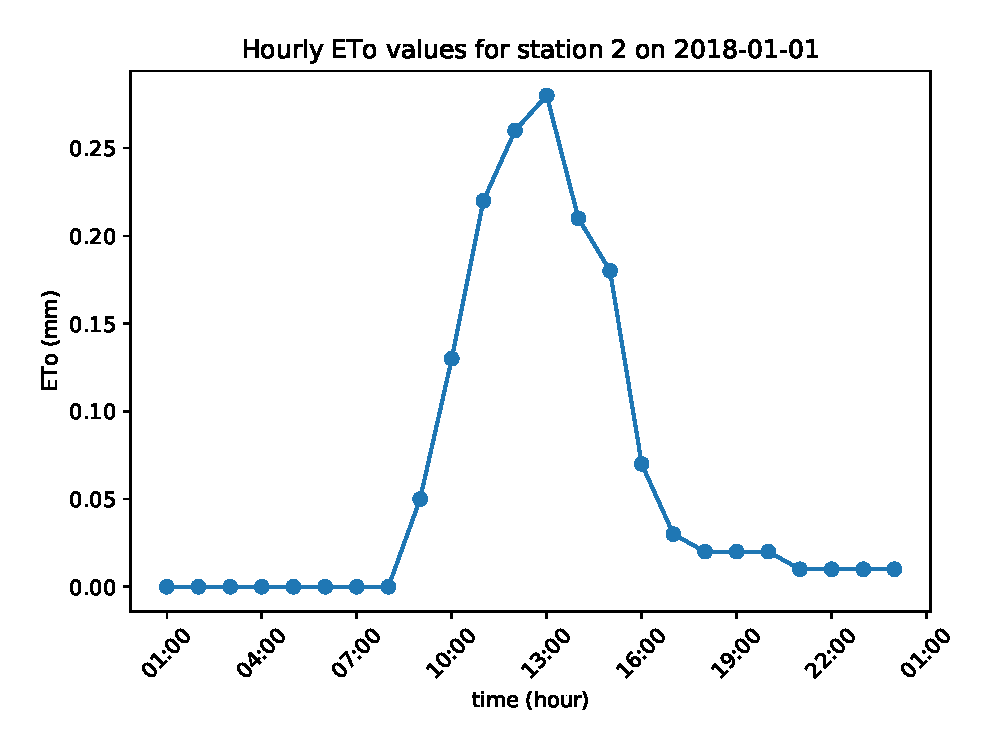
\includegraphics[width=0.9\textwidth]{images/hourly-eto-2-2018-01-01}
\end{figure}
\end{frame}

\begin{frame}
\frametitle{Mean Hourly ET Values}
\begin{figure}
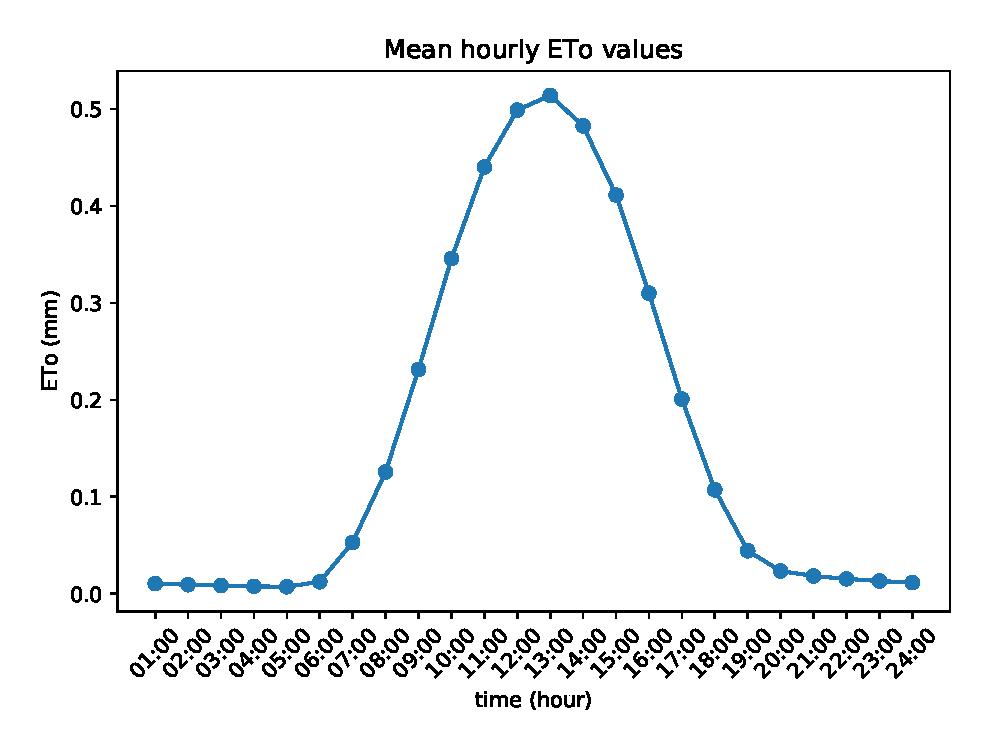
\includegraphics[width=0.9\textwidth]{images/mean-of-hourly-eto-values}
\end{figure}
\end{frame}

\begin{frame}
\frametitle{Min/Mean/Max Hourly ET Values}
\begin{figure}
	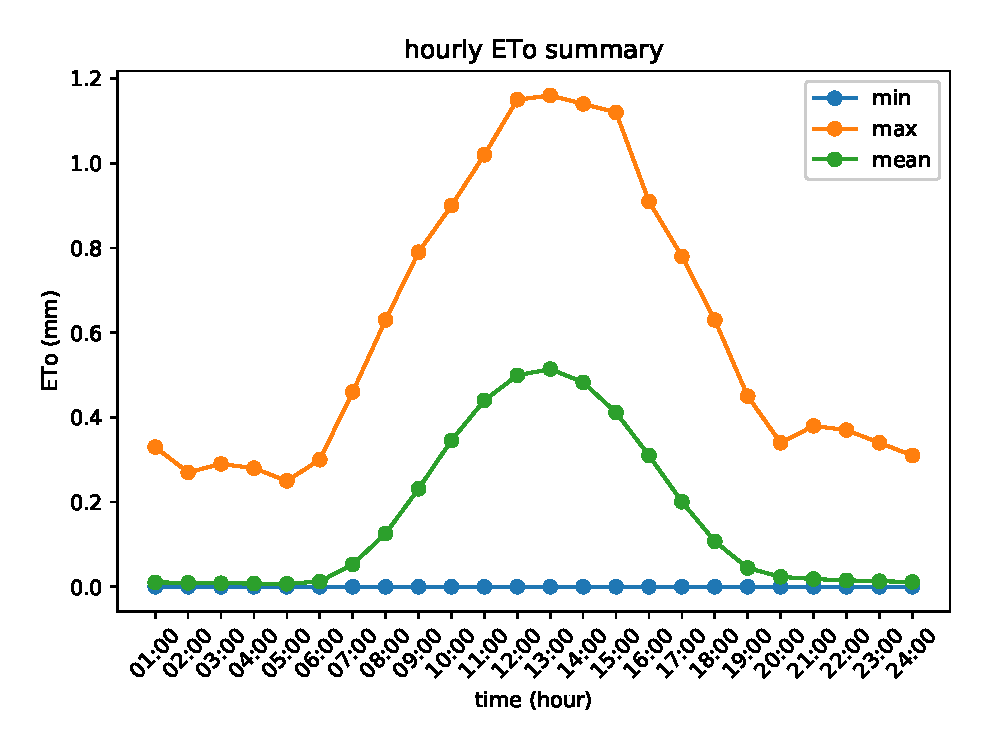
\includegraphics[width=0.9\textwidth]{images/summary-hourly-eto-values}
\end{figure}
\end{frame}

\begin{frame}
\begin{figure}
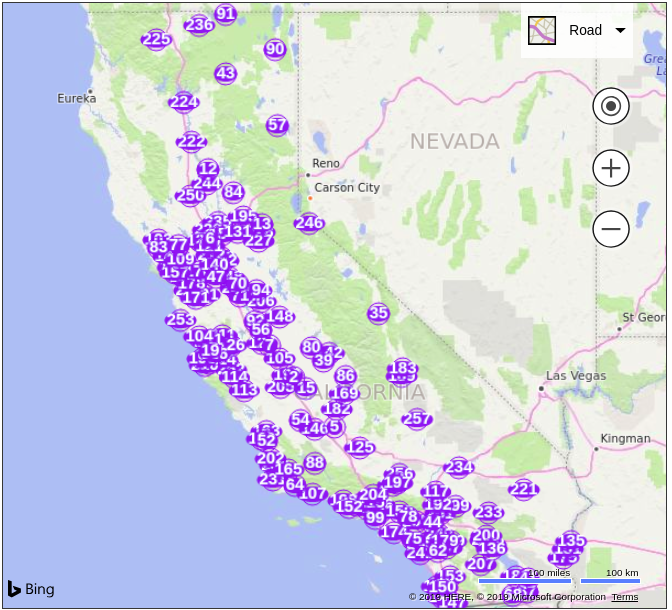
\includegraphics[width=0.8\textwidth]{images/cimis-station-location}
\end{figure}
\end{frame}

\begin{frame}
\frametitle{Stations of Interest}
\begin{itemize}
	\setlength\itemsep{1em}
	\item Station with lowest latitude $LAT_{MIN}$ (south)
	\item Station with highest latitude $LAT_{MAX}$ (north)
	\item Station with latitude closests to $\frac{LAT_{MIN}+LAT_{MAX}}{2}$ (middle)
\end{itemize}
\end{frame}

\begin{frame}
\frametitle{Mean Hourly ET Values of Stations of Interest}
\begin{figure}
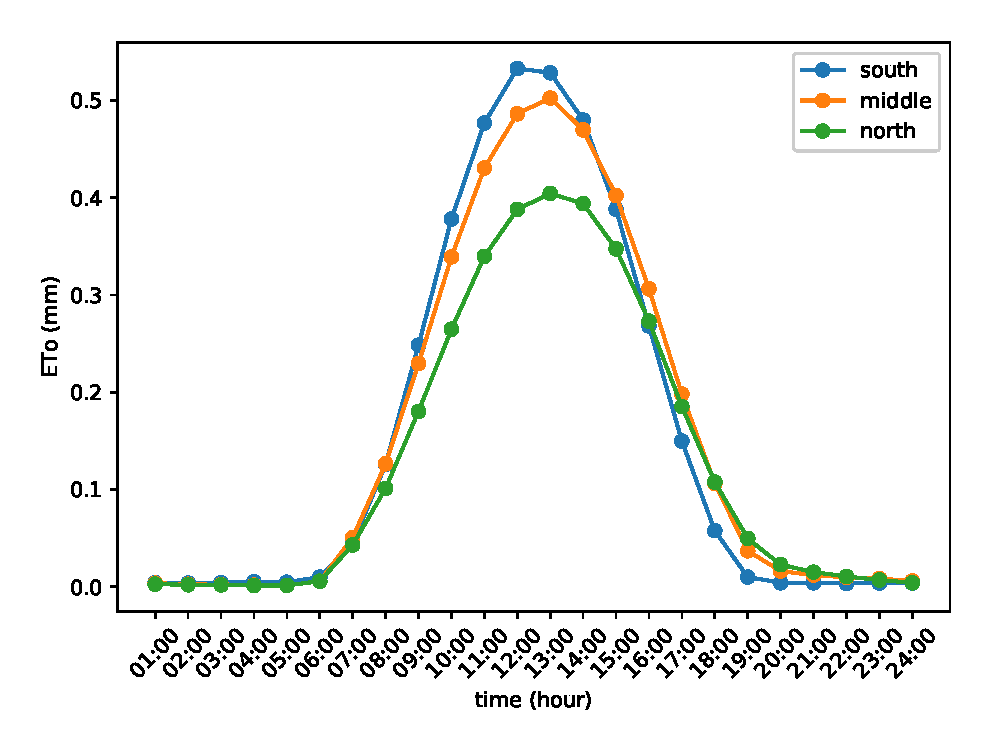
\includegraphics[width=0.9\textwidth]{images/soi-latitude-mean-of-hourly-eto-values}
\end{figure}
\end{frame}



\begin{frame}
\frametitle{Histogram of ET Values}
\begin{figure}
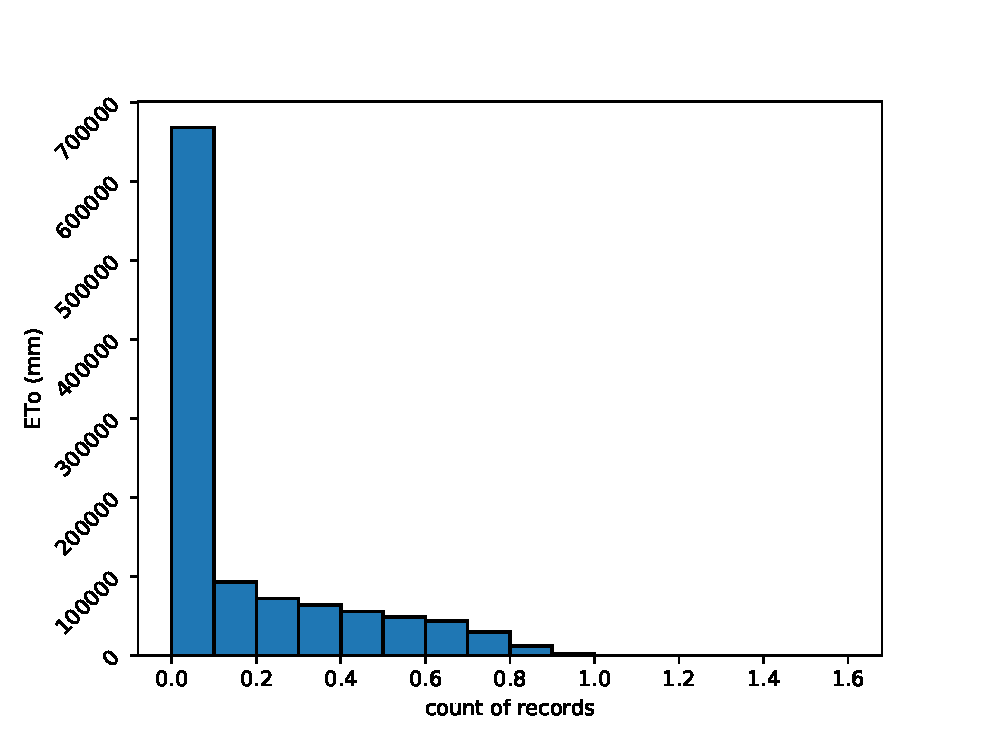
\includegraphics[width=0.9\textwidth]{images/hist-eto}
\end{figure}
\end{frame}

\begin{frame}
\frametitle{Empirical CDF of ET Values}
\begin{figure}
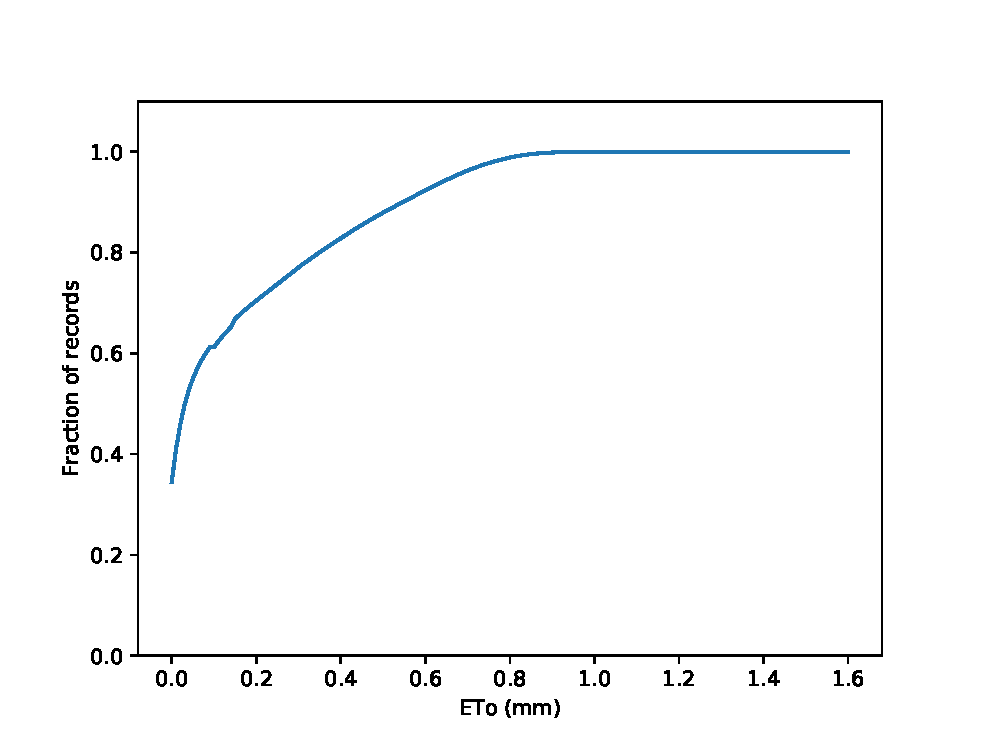
\includegraphics[width=0.9\textwidth]{images/ecdf}
\end{figure}
\end{frame}

\section{Feature Selection}


\begin{frame}
\frametitle{Correlation Analysis}
\begin{figure}
	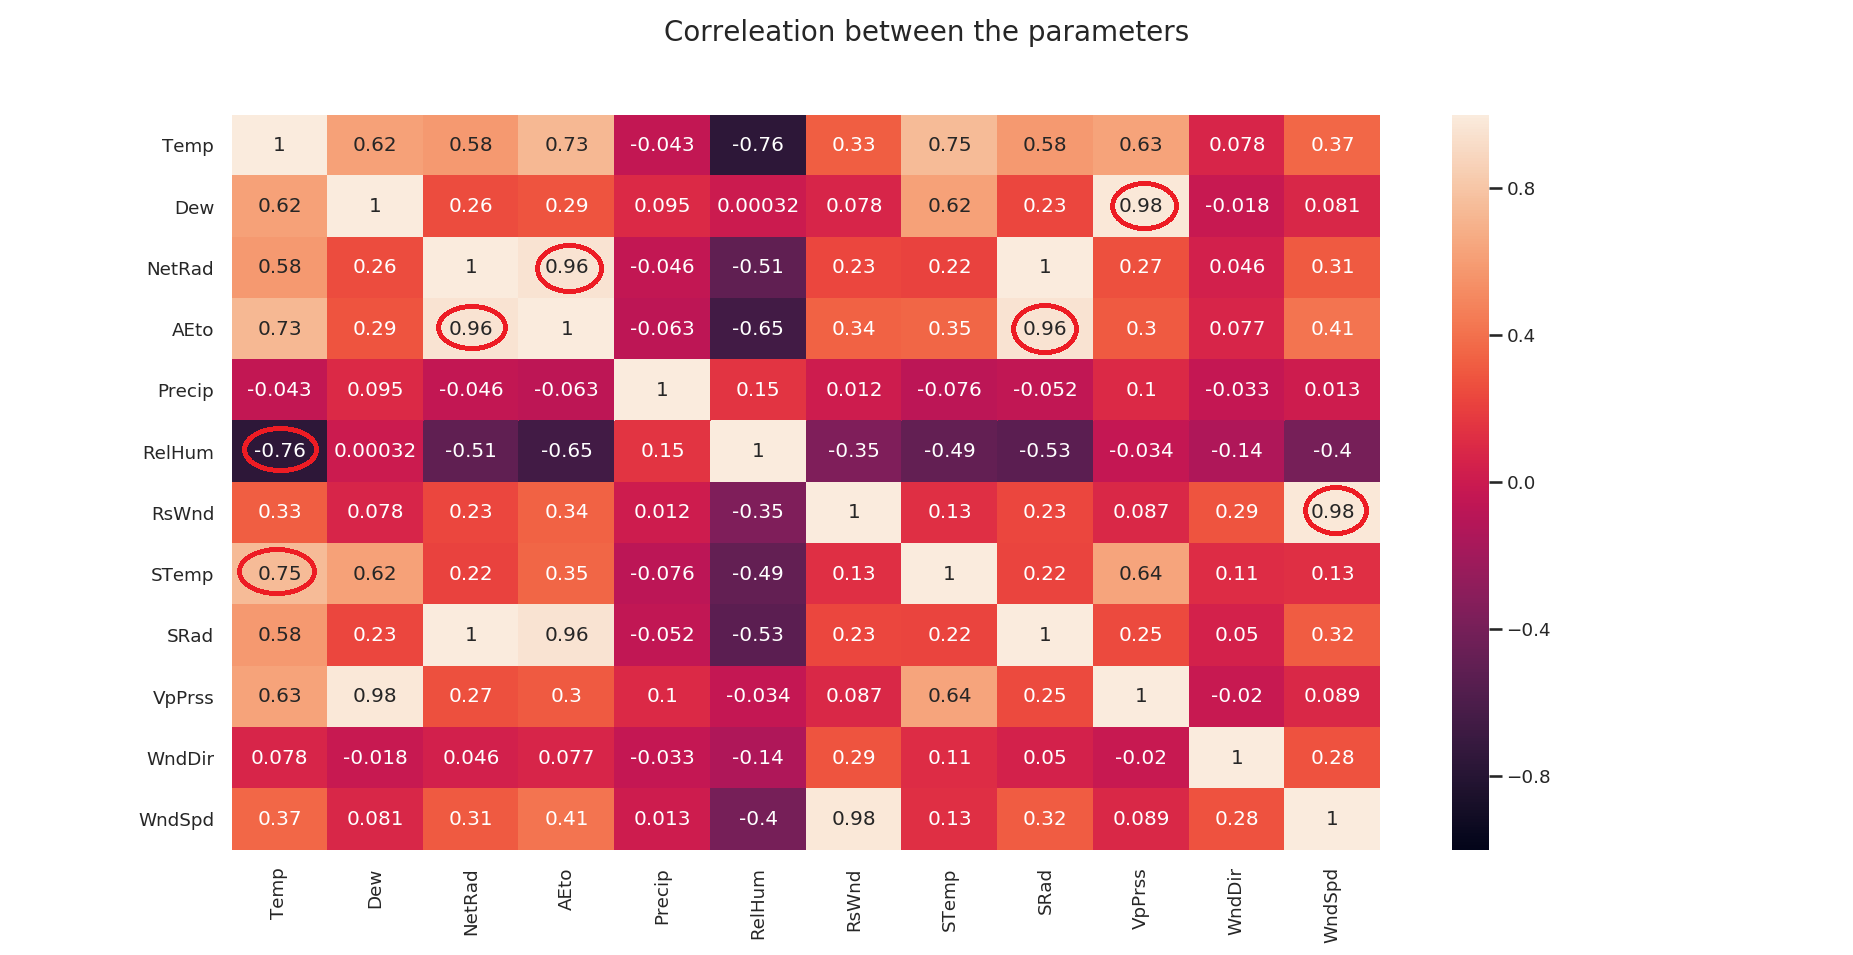
\includegraphics[width=1\textwidth]{images/correleation.png}
\end{figure}
\end{frame}

\begin{frame}
\frametitle{Biplot-all}
\begin{figure}
	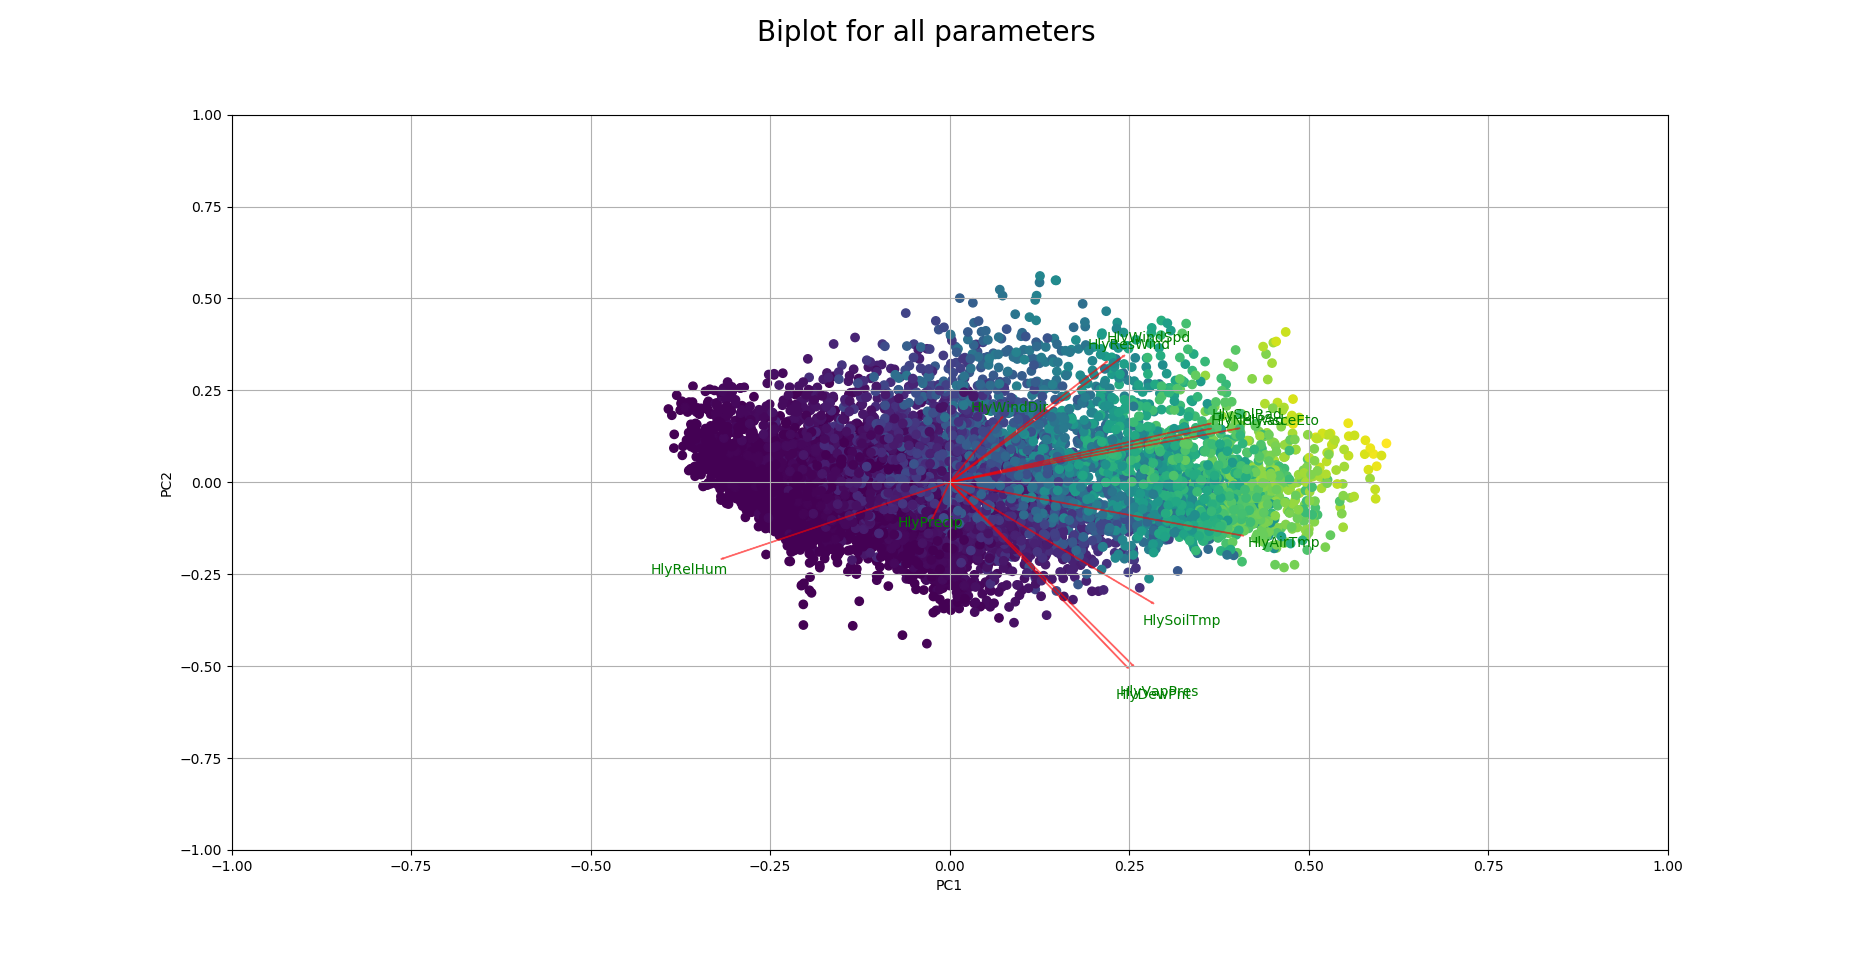
\includegraphics[width=1\textwidth]{images/biplot_full.png}
\end{figure}
\end{frame}


\begin{frame}
\frametitle{Biplot-selected}
\begin{figure}
	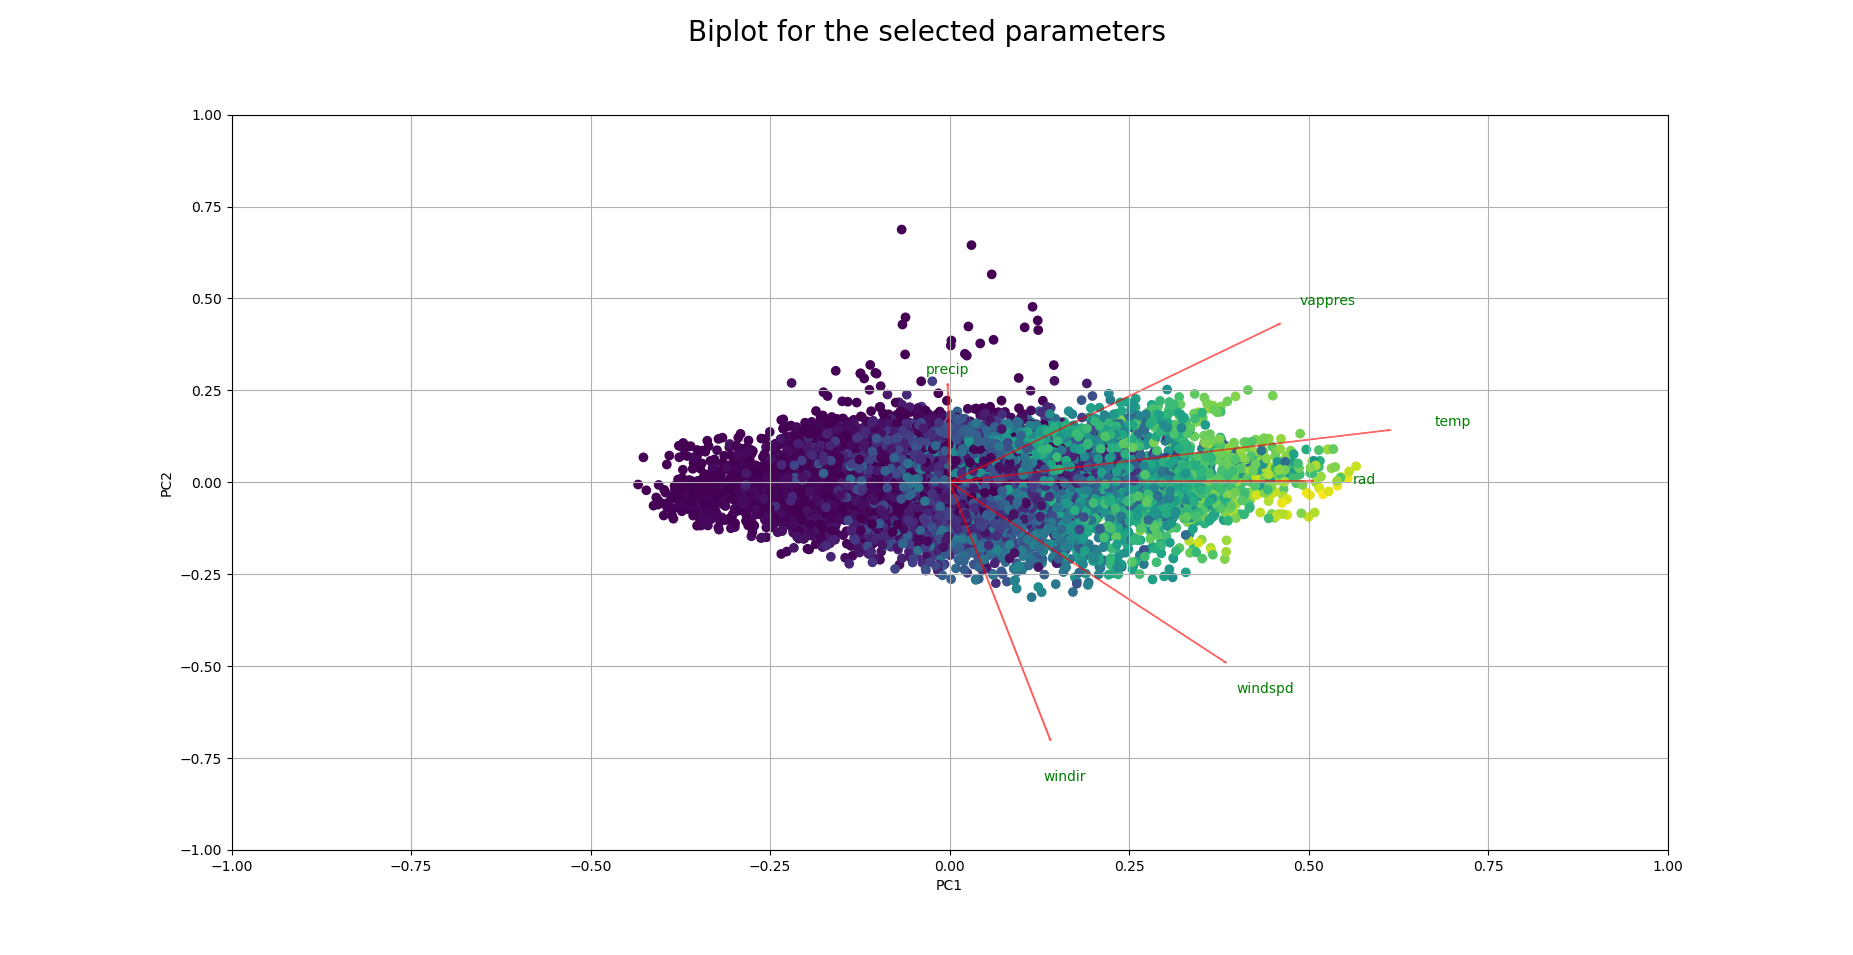
\includegraphics[width=1\textwidth]{images/biplot_selected.png}
\end{figure}
\end{frame}

\begin{frame}
\frametitle{PC1 values}
\begin{figure}
	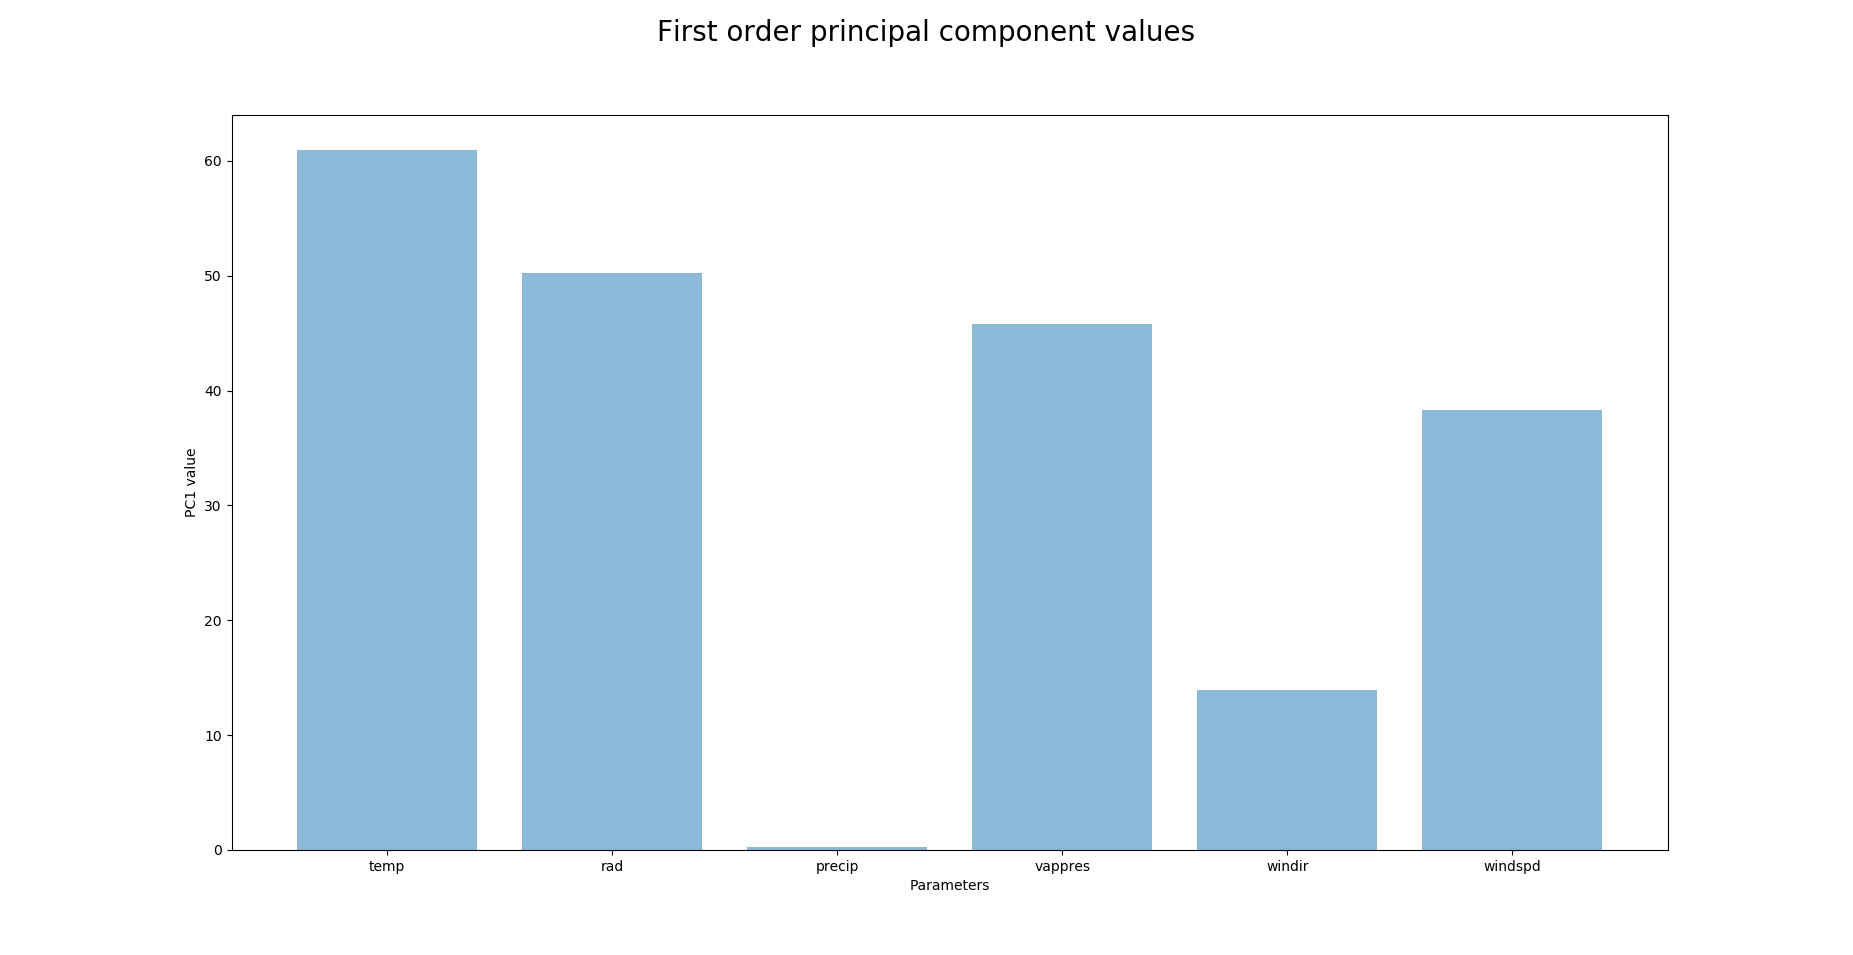
\includegraphics[width=1\textwidth]{images/PC1_values.png}
\end{figure}
\end{frame}
\section{Regression Analysis}
\begin{frame}
\frametitle{Estimation of ET Values}
\tikzproblem{Given a set of features, can we estimate ET?}
\begin{itemize}
\setlength\itemsep{1em}
\item Which features to choose?
\item \textit{How well} is our estimate?
\end{itemize}
\end{frame}

\begin{frame}
\frametitle{(CIMIS) Penman Monteith Equation for Calculating ET}
\begin{equation*}
\boxed{ET_o = \frac{\bigtriangleup(R_n-G)}{\lambda[\bigtriangleup+\gamma(1+C_du_2)]} + \frac{\gamma\frac{37}{T_a+273.16}u_2(e_s-e_a)}{\bigtriangleup+\gamma(1+C_du_2)}}
\end{equation*}
\tikzstatement{Ultimately depends on four weather features}
\begin{itemize}
\setlength\itemsep{1em}
\item Solar net radiation
\item Vapor pressure
\item Air temperature
\item Wind speed
\end{itemize}
\end{frame}

\begin{frame}
\frametitle{Scatterplot Matrix of Features of Interest}
\begin{figure}
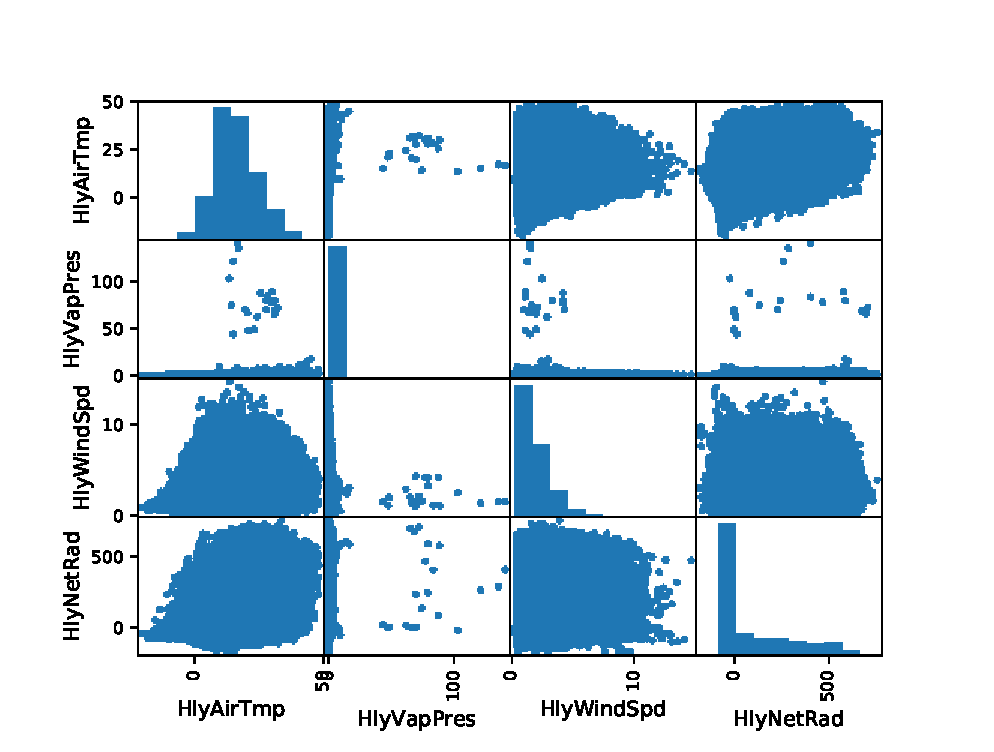
\includegraphics[width=0.85\textwidth]{images/scatterplot-matrix-HlyAirTmp-HlyVapPres-HlyWindSpd-HlyNetRad}
\end{figure}
\end{frame}

\begin{frame}
\frametitle{Regression Results}
\footnotesize
\begin{tabular}{|l|l|l|}
\hline
\textbf{Features} & \textbf{Mean Squared Error} & \textbf{$R^2$ Value}\\
\hline
HlyAirTmp,HlyNetRad,HlyVapPres,HlyWindSpd & 0.000970123960314 & 0.981294016164\\
\hline
HlyAirTmp,HlyNetRad,HlyVapPres & 0.00130358866256 & 0.974761220654\\
\hline
HlyAirTmp,HlyNetRad,HlyWindSpd & 0.00131186536214 & 0.974527982555\\
\hline
HlyAirTmp,HlyNetRad & 0.00173654973306 & 0.966537004752\\
\hline
HlyNetRad,HlyVapPres,HlyWindSpd & 0.00248645097725 & 0.952009857384\\
\hline
HlyNetRad,HlyWindSpd & 0.0024909080494 & 0.951659909255\\
\hline
HlyNetRad,HlyVapPres & 0.00302176798112 & 0.941065800356\\
\hline
HlyNetRad & 0.00304665078019 & 0.940955854127\\
\hline
HlyAirTmp,HlyVapPres,HlyWindSpd & 0.0236668111725 & 0.540318481\\
\hline
HlyAirTmp,HlyWindSpd & 0.0242823252297 & 0.528560618195\\
\hline
HlyAirTmp,HlyVapPres & 0.026563048828 & 0.485028160007\\
\hline
HlyAirTmp & 0.0278295291341 & 0.459710153733\\
\hline
HlyVapPres,HlyWindSpd & 0.0407552684279 & 0.208827525819\\
\hline
HlyWindSpd & 0.0412914020576 & 0.196118554063\\
\hline
HlyVapPres & 0.0510006461517 & 0.0128578989128\\
\hline
\end{tabular}
\end{frame}

\section{Nearest Neighbor Analysis}
\begin{frame}
\frametitle{Nearest Neighbor Analysis}
\tikzproblem{Given the ET value of $k$ nearest stations of a place, can we estimate ET?}
\begin{itemize}
\setlength\itemsep{1em}
\item Arithmetic mean of $k$ values
\item Inverse Distance Weighted (IDW) average of $k$ values
\end{itemize}
\end{frame}

\begin{frame}
\begin{figure}
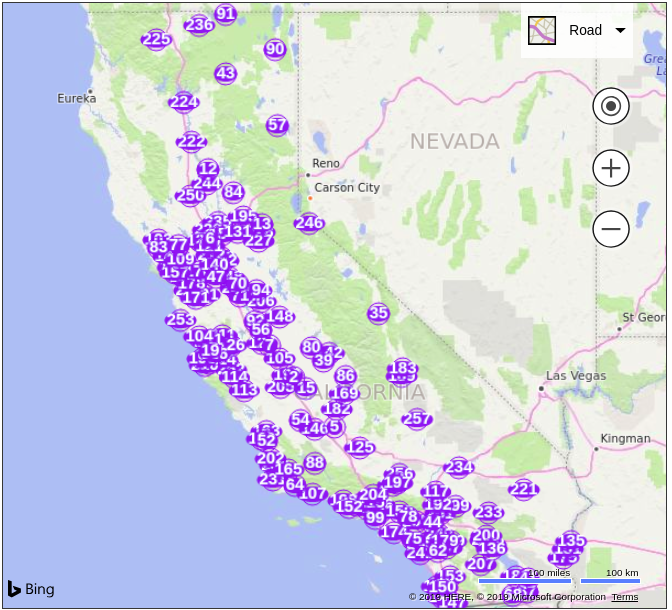
\includegraphics[width=0.8\textwidth]{images/cimis-station-location}
\end{figure}
\end{frame}

\begin{frame}
\frametitle{Stations of Interest}
\begin{itemize}
	\setlength\itemsep{1em}
	\item Station with lowest distance $D_{MIN}$ to nearest neighbor
	\item Station with highest distance $D_{MAX}$ to nearest neighbor
	\item Station with nearest neighbor at a distance closest to $\frac{D_{MIN}+D_{MAX}}{2}$
\end{itemize}
\end{frame}

\begin{frame}
\frametitle{Nearest Neighbor Results}
\centering
\footnotesize
\begin{tabular}{|l|l|l|l|}
\hline
\textbf{Station Number} & \textbf{Num of Neighbors} & \textbf{MSE for Average} &\textbf{MSE for IDW}\\
\hline
129 & 1 & 0.000832971114168 & 0.000832971114168\\
\hline
234 & 1 & 0.00437018526497 & 0.00437018526497\\
\hline
57 & 1 & 0.00451400872516 & 0.00451400872516\\
\hline
129 & 2 & 0.00116361600992 & 0.000620877927137\\
\hline
234 & 2 & 0.00761026004119 & 0.00730456269316\\
\hline
57 & 2 & 0.00371994564336 & 0.0037154634375\\
\hline
129 & 3 & 0.000890784115612 & 0.000596760525931\\
\hline
234 & 3 & 0.00908058999082 & 0.00863260116925\\
\hline
57 & 3 & 0.00335367604618 & 0.00334925237208\\
\hline
129 & 4 & 0.00116647617403 & 0.00063999172153\\
\hline
234 & 4 & 0.00919325287807 & 0.00878339044833\\
\hline
57 & 4 & 0.00361403432169 & 0.00357201358681\\
\hline
\end{tabular}
\end{frame}

\begin{frame}
\begin{figure}
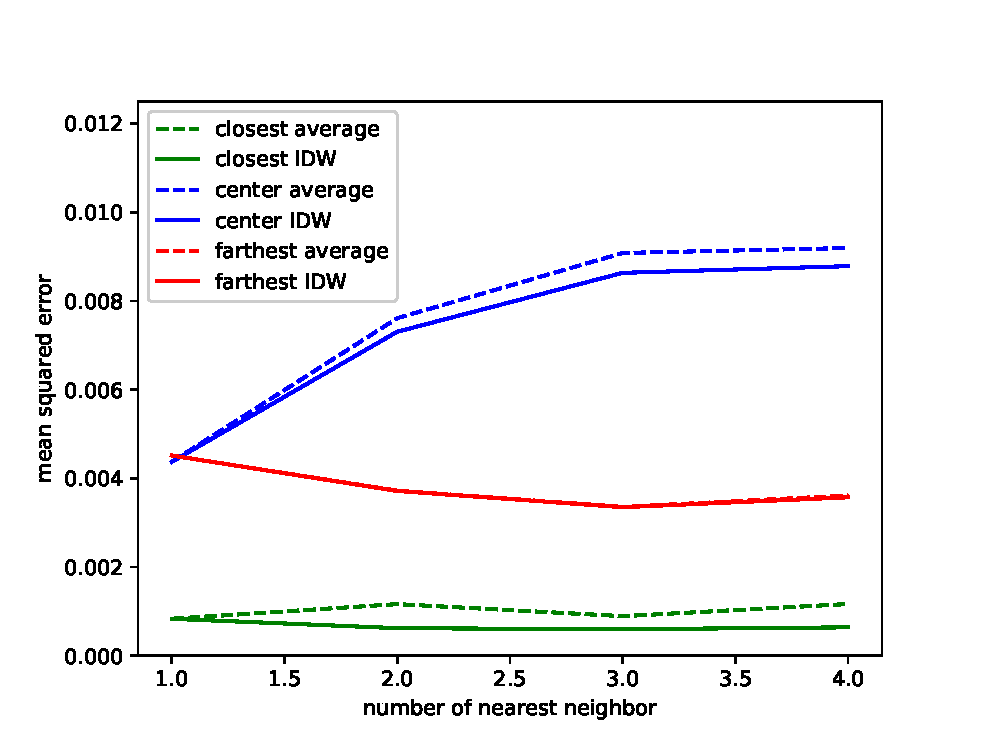
\includegraphics[width=1.0\textwidth]{images/soi-nearest-distance}
\end{figure}
\end{frame}

\begin{frame}
\frametitle{A Different Approach to Nearest Neighbor}
\begin{itemize}
\setlength\itemsep{1em}
\item Some stations are sparsely located, some are densely located
\item Distance to $n$th nearest station for different stations might vary widely
\end{itemize}
\tikzproblem{What is an optimal value of $R$ such that $k\prime$ stations\\ within that radius gives best overall estimates?}
\tikzsolution{future work $\ldots$}
\end{frame}

\section{Demo}
\begin{frame}
	\begin{center}
		{\fontsize{20}{20}\selectfont
			\textbf{DEMO}
		}
	\end{center}
\end{frame}

\begin{frame}
\frametitle{Demo}
We developed a Python webapp using Flask to display all the active CIMIS stations in California. You can hover over any station and a popup shows the ET values for that station, for all the months of year 2018. We used Leaflet library for creating the interactive maps. You can also select a station, pick a date and get the ET values for that particular date. 
\end{frame}

\begin{frame}
	\frametitle{CIMIS stations}
	\centering
	\begin{figure}
		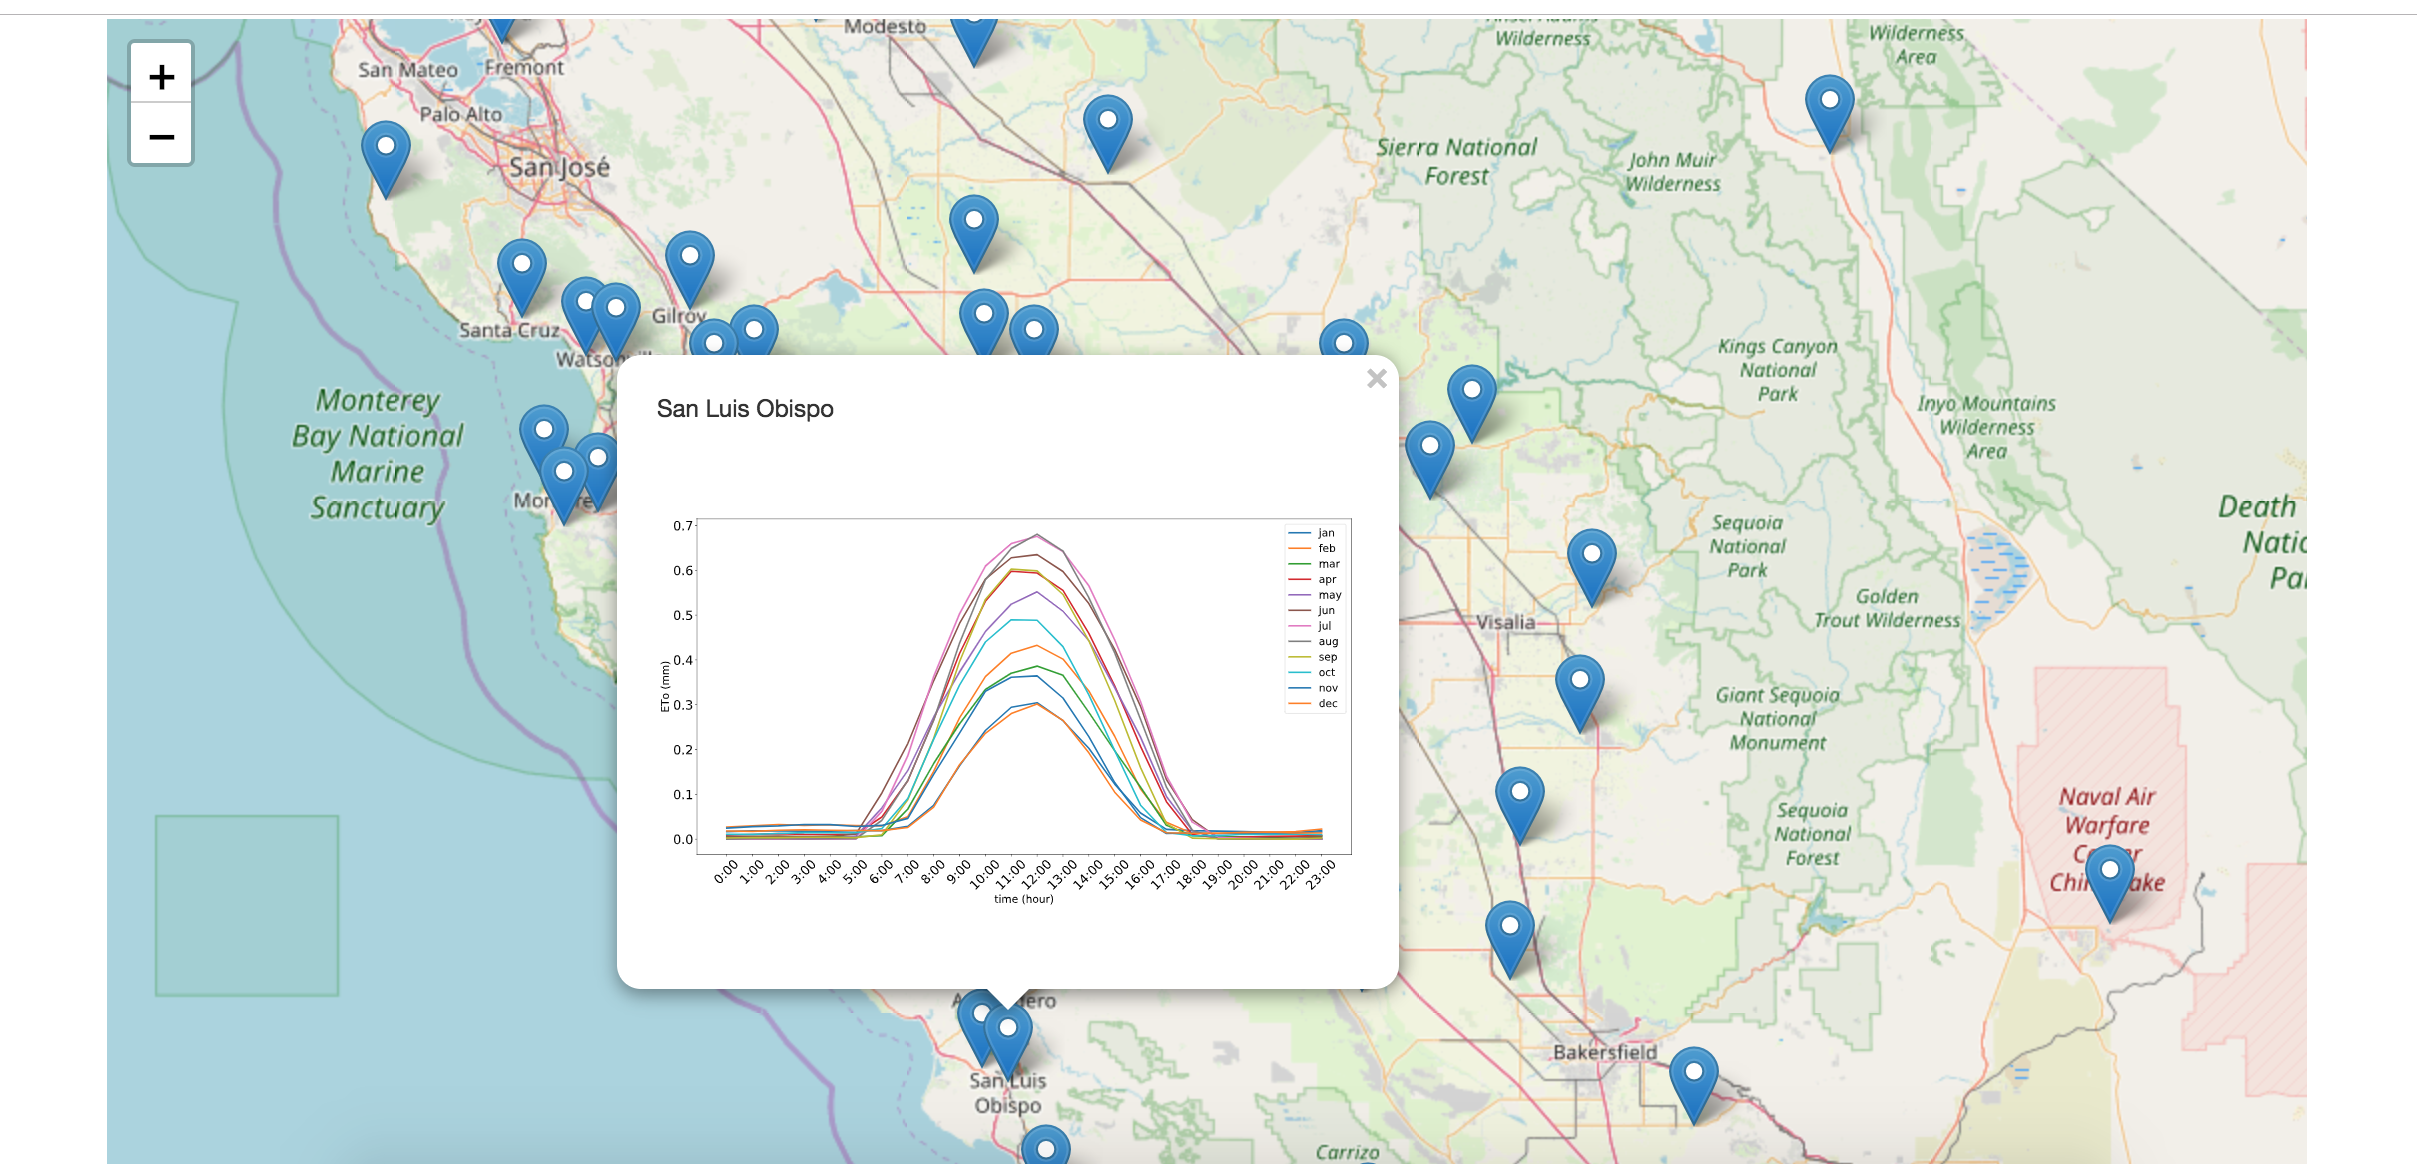
\includegraphics[width=0.9\textwidth]{images/fig1.png}
		\caption{Graph showing the monthly ET values for San Luis Obispo}\label{fig:fig1}
	\end{figure}
\end{frame}

\begin{frame}
	\frametitle{ET values on a particular date}
	\centering
	\begin{figure}
		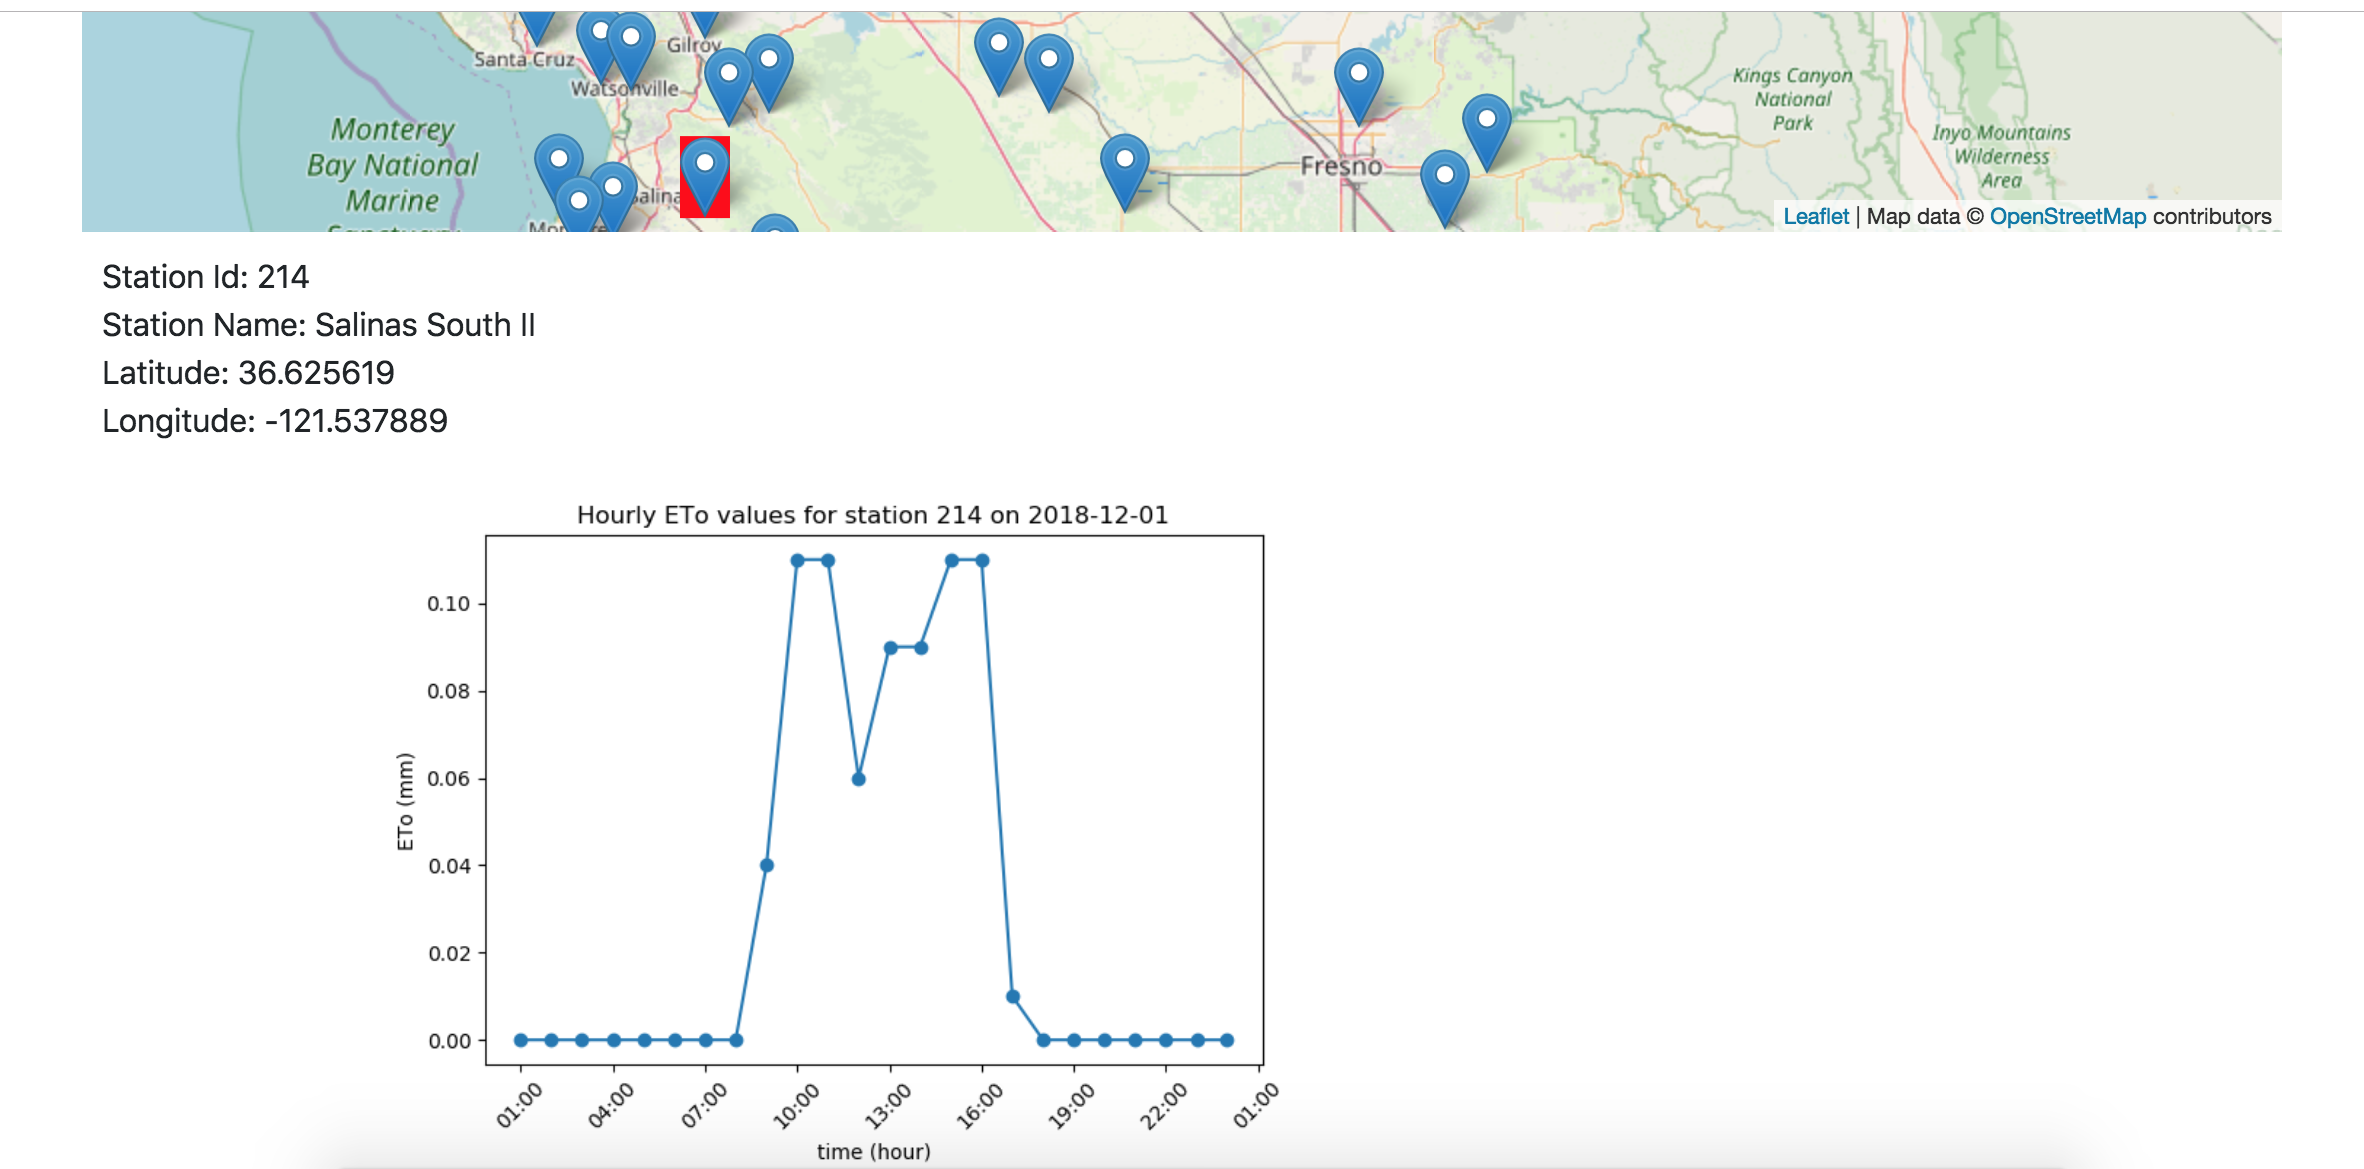
\includegraphics[width=0.9\textwidth]{images/fig2.png}
	\end{figure}
\end{frame}

\begin{frame}
	\frametitle{Linear Regression}
	\centering
	\begin{figure}
		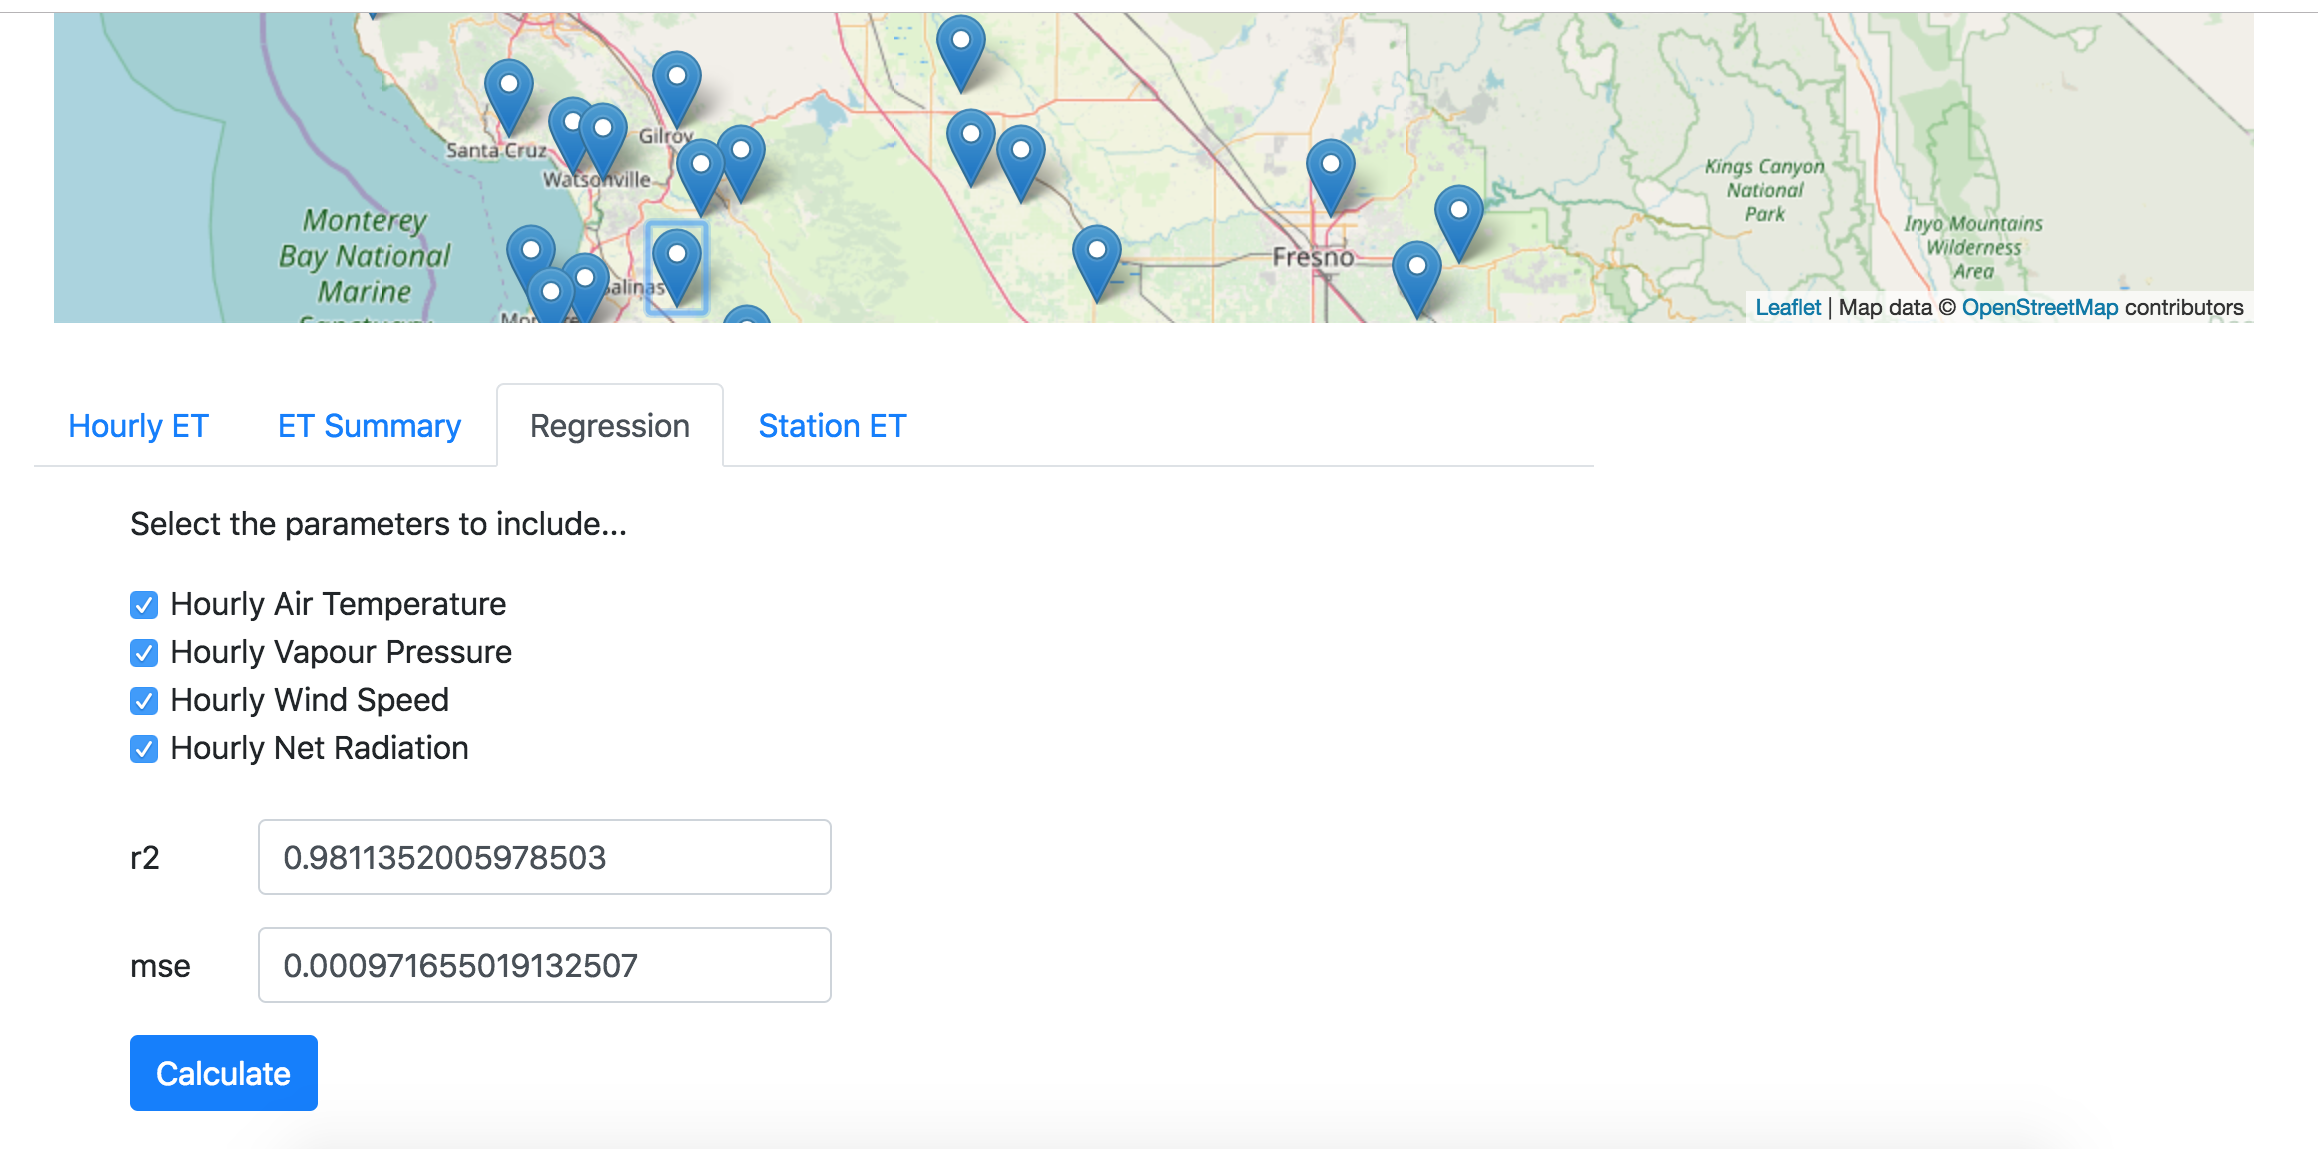
\includegraphics[width=0.9\textwidth]{images/fig3.png}
	\end{figure}
\end{frame}

\begin{frame}
	In Fig.~\ref{fig:2-2016} we can see an example of the typical 12 month graph for one of the stations. There is a even spread between all the months in average hourly ET values and a smooth curve through the day. We can see that as we expected in the winter months ET values are lower than in the summer. There is a small amount of evapo-transpiration over the night which is not unusual but is not the case for all stations. 
\end{frame}

\begin{frame}
\frametitle{Normal 12-month Graph for Station 2 in 2016}
\centering
\begin{figure}
	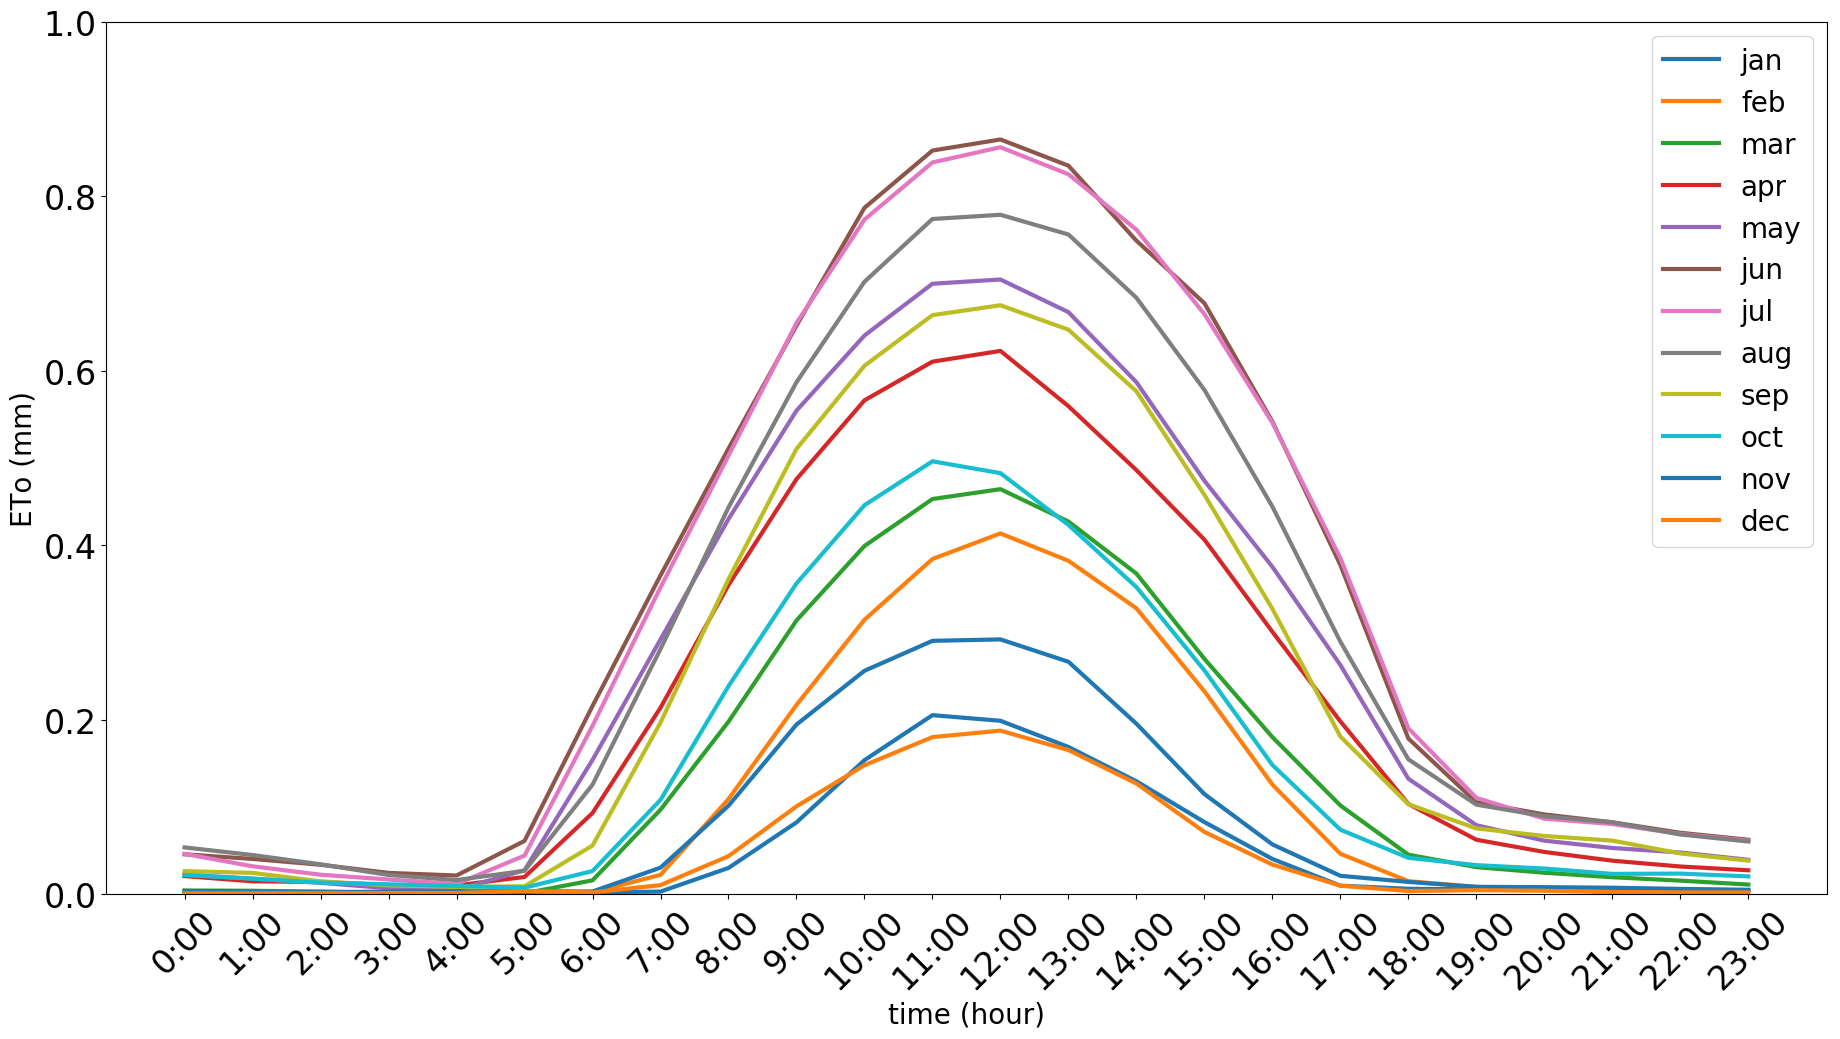
\includegraphics[width=0.9\textwidth]{images/2-2016.png}
	\caption{Normal 12-month Graph for Station 2 in 2016}\label{fig:2-2016}
\end{figure}
\end{frame}

\begin{frame}
	If we take a sampling of the all graphs produced from the many stations we see four different stations types. In Fig.~\ref{fig:12-2016} we see an example of the second category where there is a clear split between the winter and summer months. If we look at the graphs for stations like this through the years we can see that there is consistently a split between months but which months varies between years. In future work we could predict when this jump in ET values occurs to help farmers prepare to the increase in water needs. 
\end{frame}

\begin{frame}
\frametitle{12-month Graph for Station 12 in 2016}
\centering
\begin{figure}
	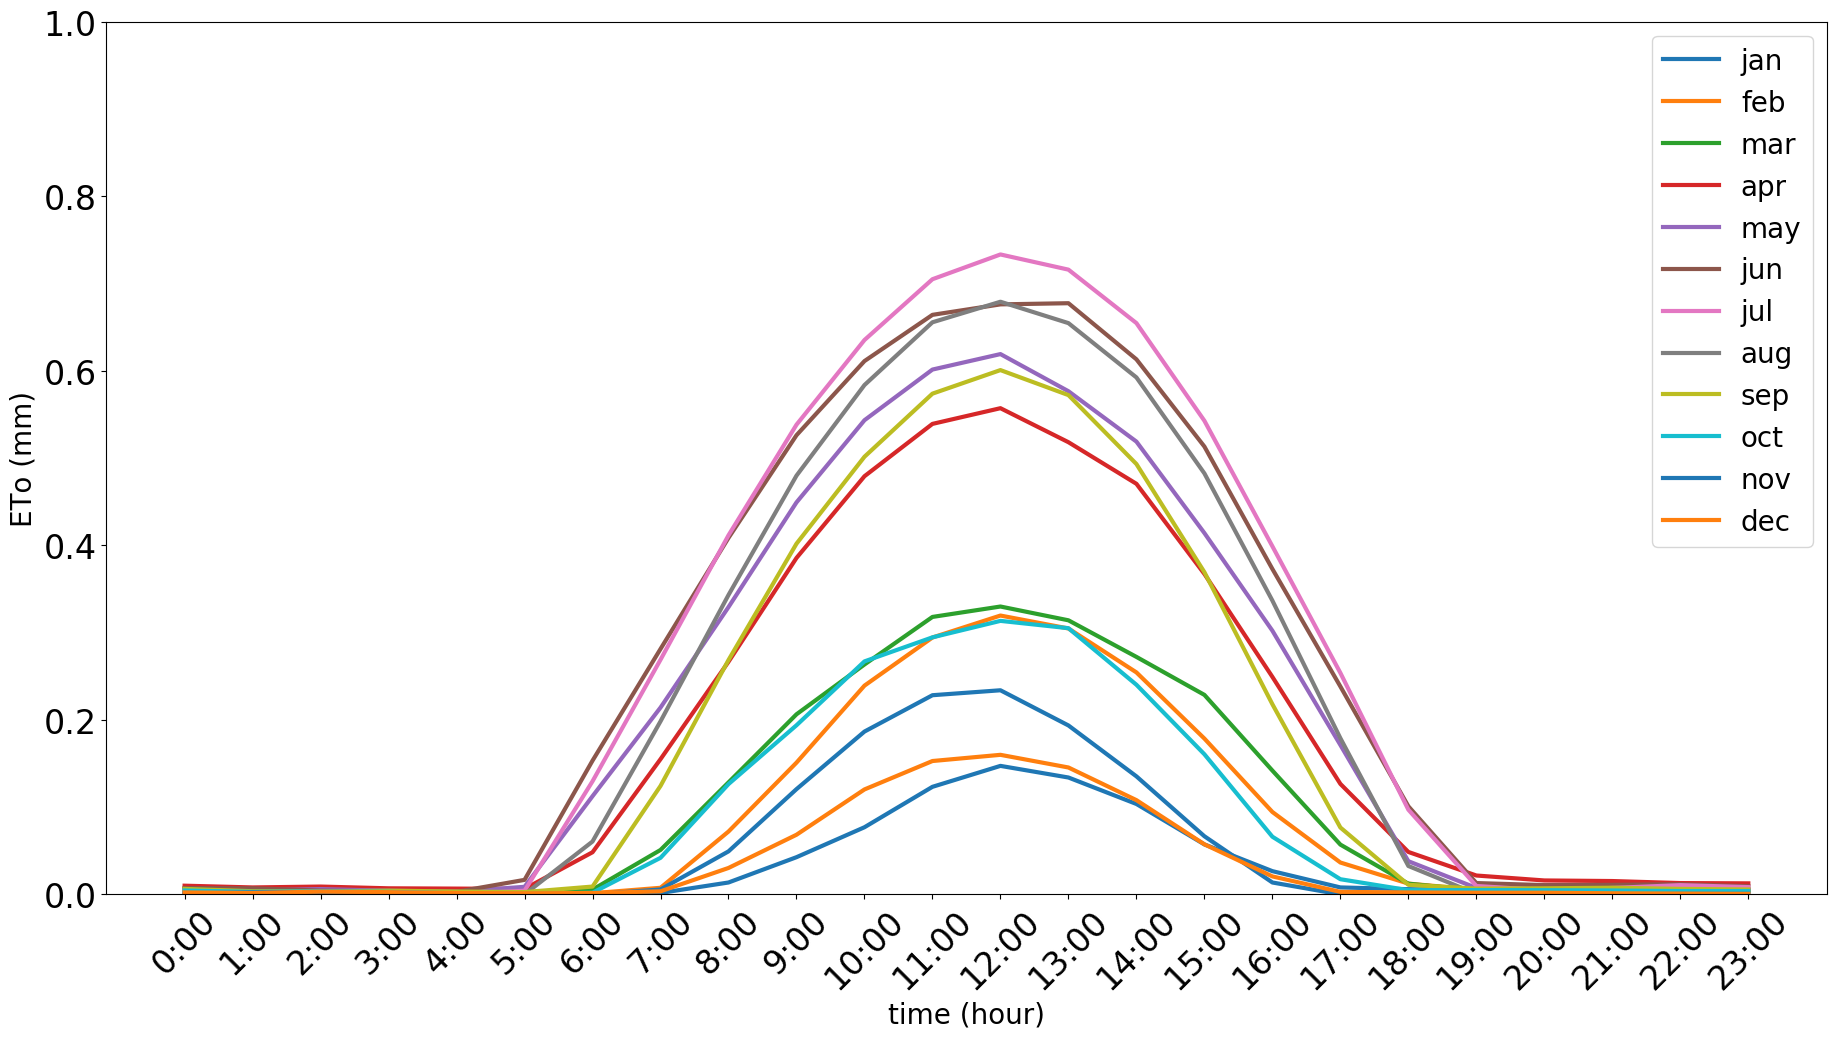
\includegraphics[width=0.9\textwidth]{images/12-2016.png}
	\caption{12-month Graph for Station 12 in 2016}\label{fig:12-2016}
\end{figure}
\end{frame}

\begin{frame}
	Here We can see an example (Fig.~\ref{fig:62-2018}) of an anomaly in the day where unexpectedly in the night the ET values start increasing. We don't know why this occurred but could be a sensor error or some large change in the local environment that cause ET to increase in the night.
\end{frame}

\begin{frame}
\frametitle{12-month Graph for Station 62 in 2018}
\centering
\begin{figure}
	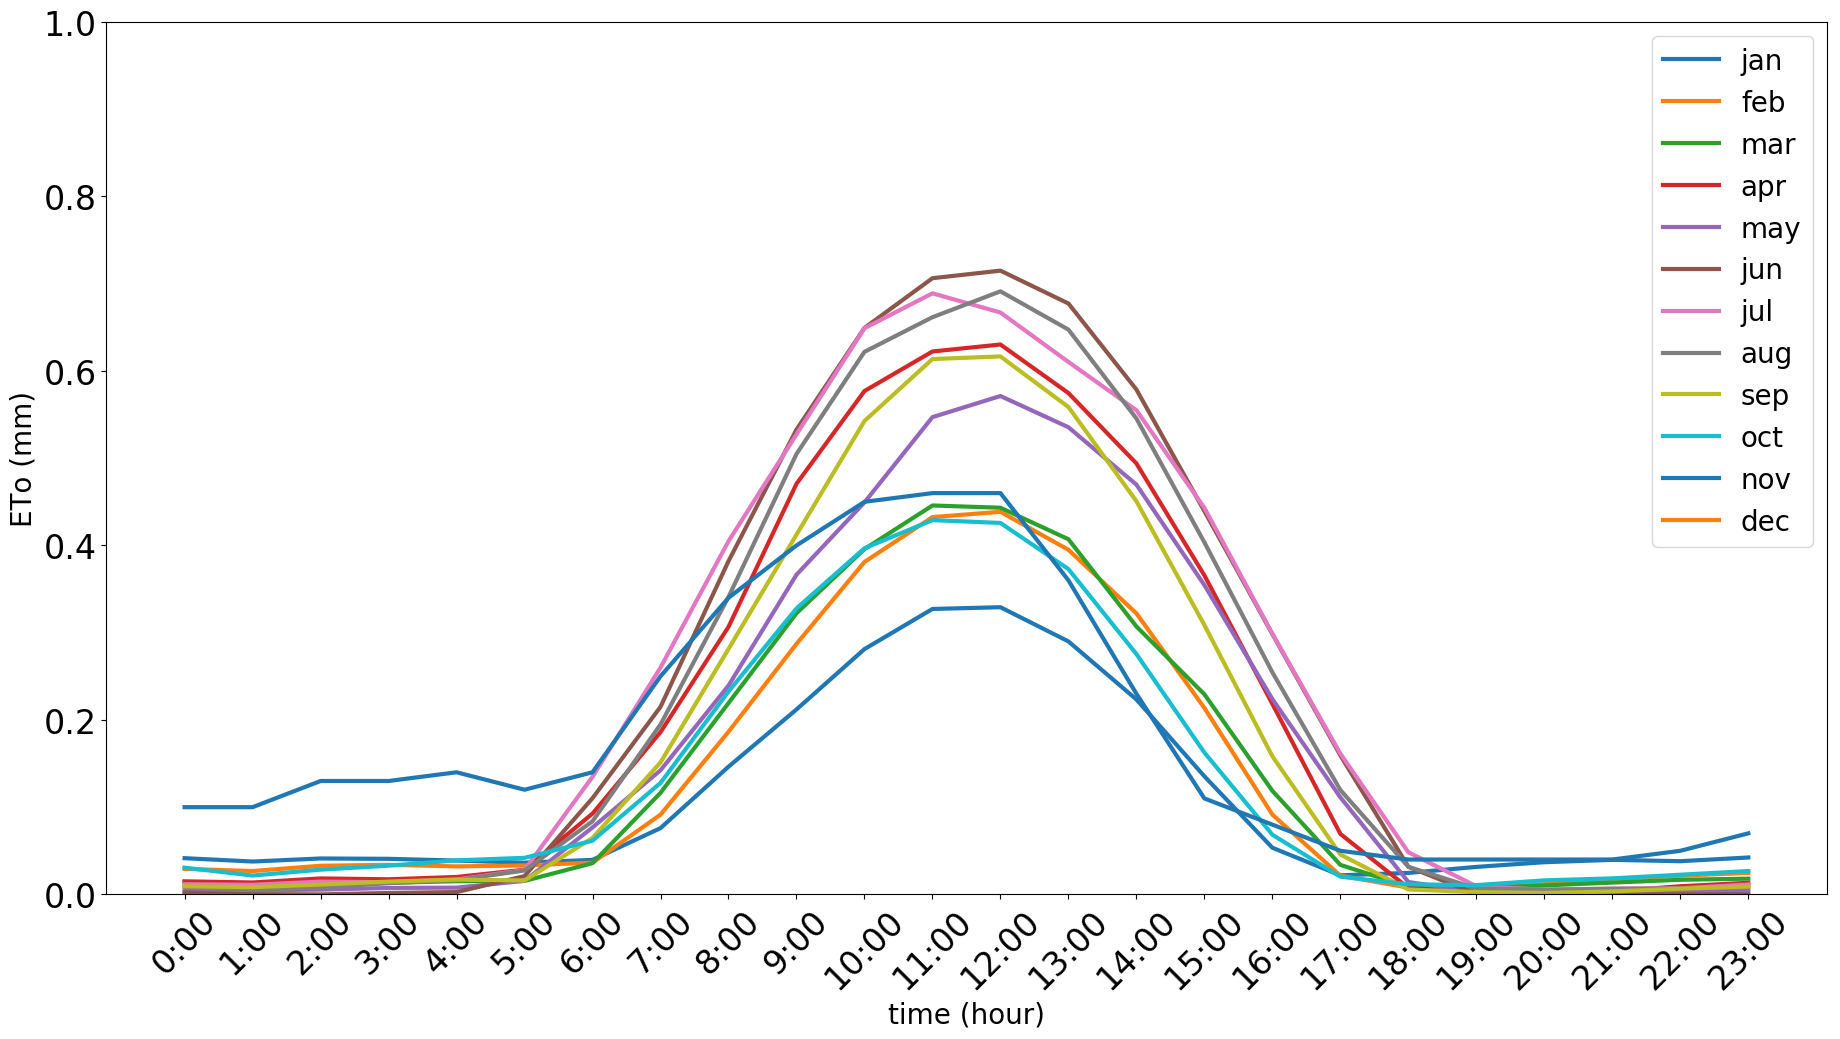
\includegraphics[width=0.9\textwidth]{images/62-2018.png}
	\caption{12-month Graph for Station 12 in 2016}\label{fig:62-2018}
\end{figure}
\end{frame}

\begin{frame}
	In Fig.~\ref{fig:234multi} we have a 3 year composite graph for 2016, 2017 and 2018. This particular station is an example of a location with a large tail of ET values that continues late into the night. We also see a trend where the ET values decrease between the years of 2016-2018. This could be an indication of a environmental that greatly reduced the water loss in the vicinity of that stations.
\end{frame}

\begin{frame}
\frametitle{36-month Graph for Station 234}
\centering
\begin{figure}
	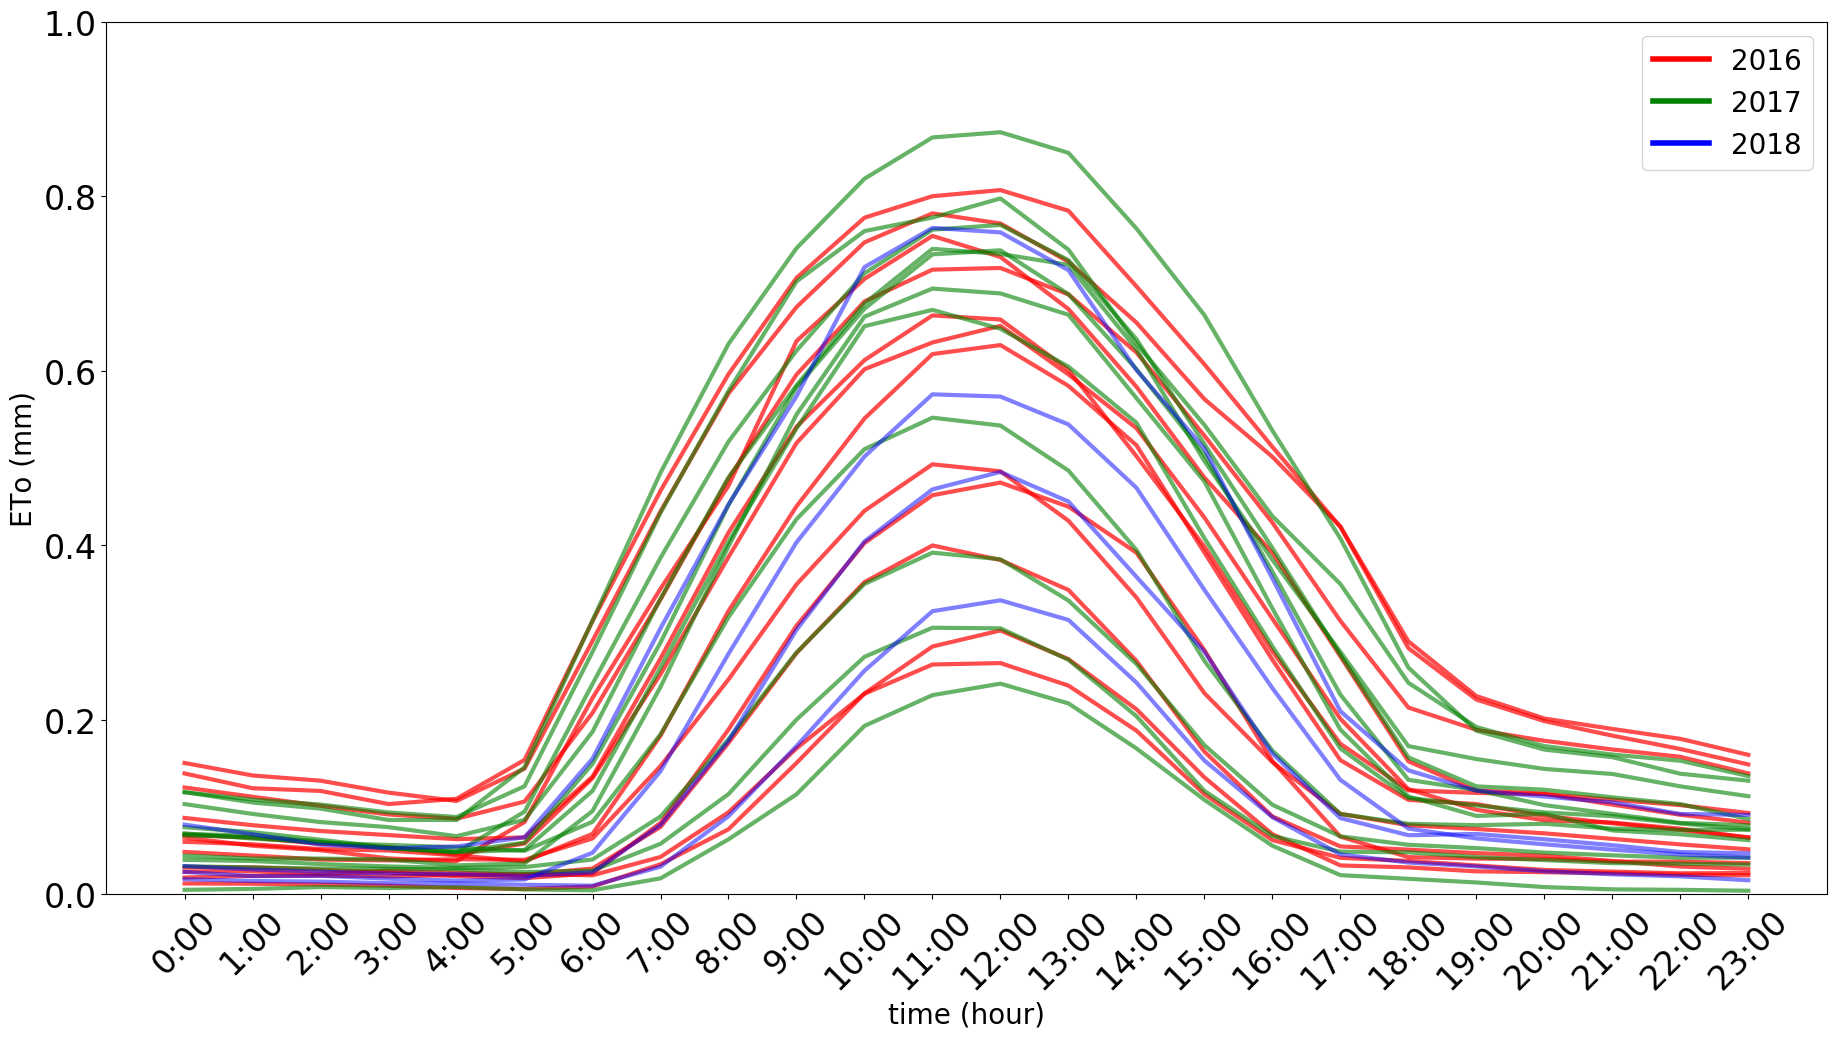
\includegraphics[width=0.9\textwidth]{images/234multi.png}
	\caption{36-month Graph for Station 234}\label{fig:234multi}
\end{figure}
\end{frame}

\begin{frame}
	Looking through the 3 years graphs for the stations we see an interesting trend for station 7 (Fig.~\ref{fig:7multi}). There is a dip in ET values during the winter months at 10am. We investigate the cause of this dip and we saw that there was a similar shape in the hourly solar radiation graph(Fig.~\ref{fig:solar}). Looking at the google maps location for stations 7 we can see that a tree would block the sensor in the winter when the sun is at a lower angle.
\end{frame}

\begin{frame}
\frametitle{36-month Graph for Station 7}
\centering
\begin{figure}
	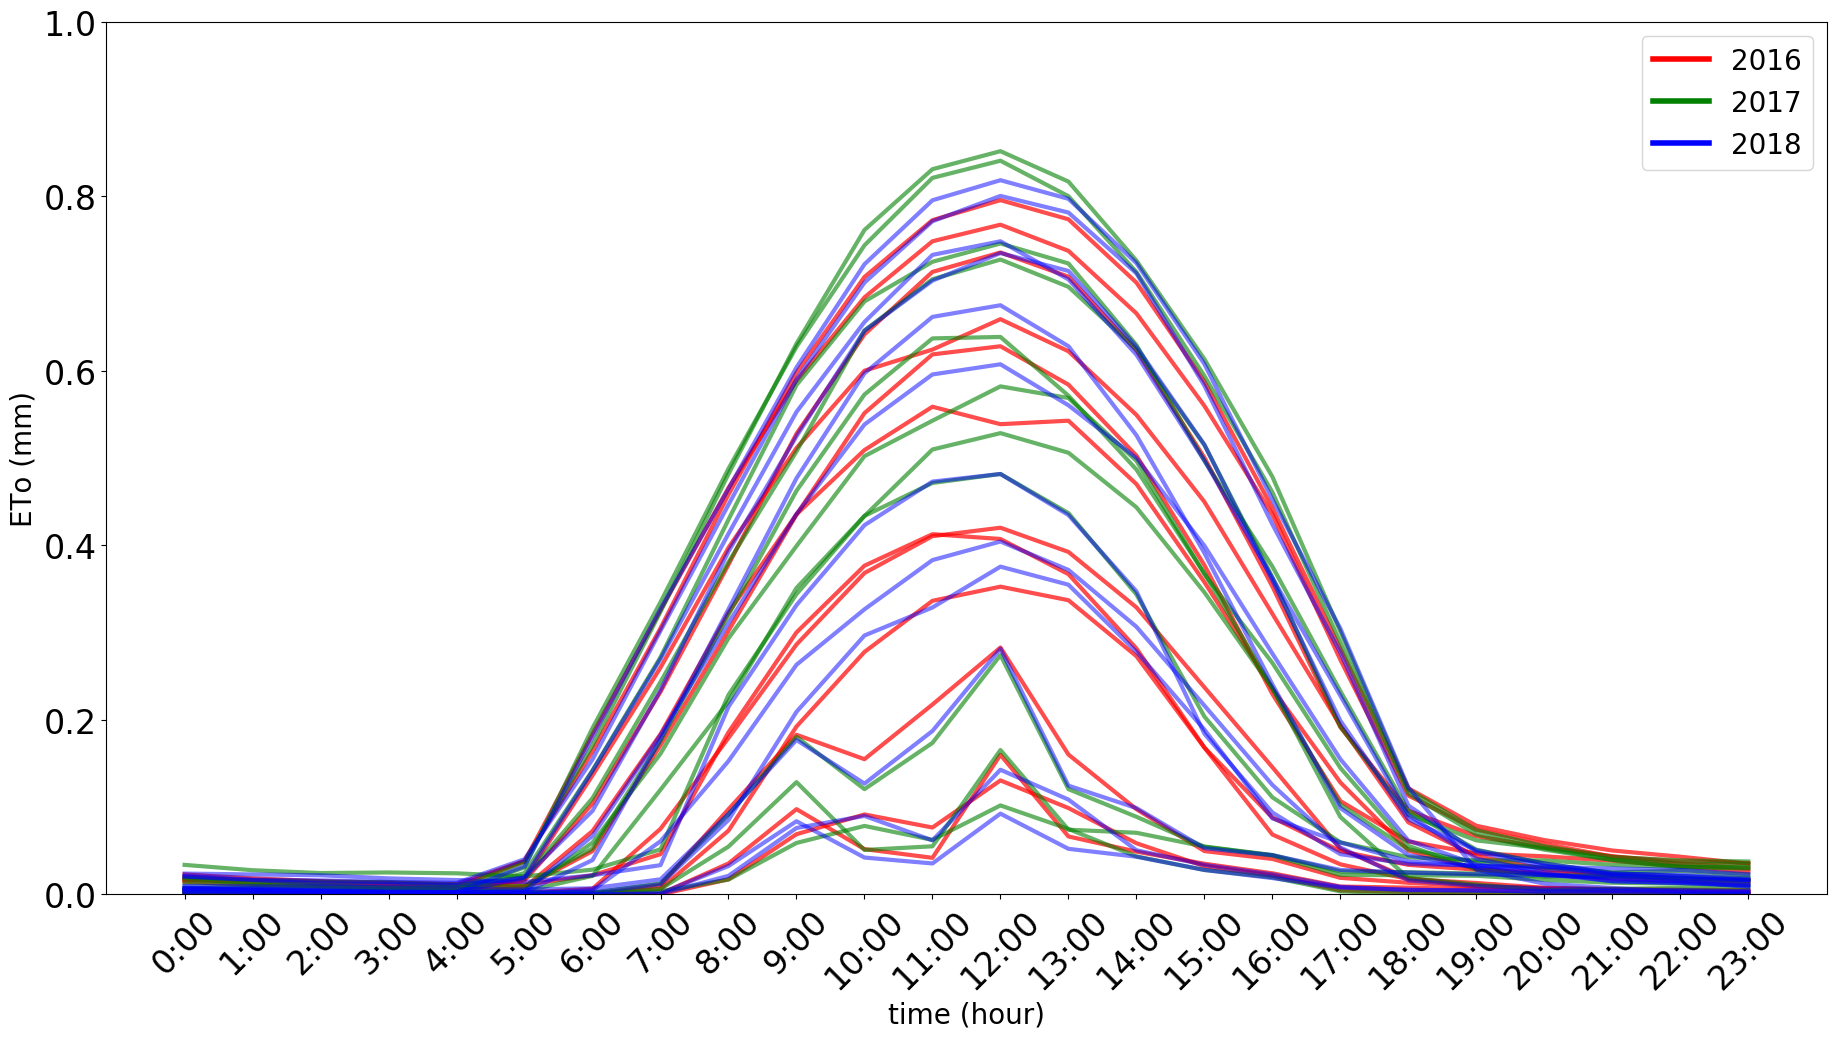
\includegraphics[width=0.9\textwidth]{images/7multi.png}
	\caption{36-month Graph for Station 7}\label{fig:7multi}
\end{figure}
\end{frame}


\begin{frame}
\frametitle{36-month Solar Graph for Station 7}
\centering
\begin{figure}
	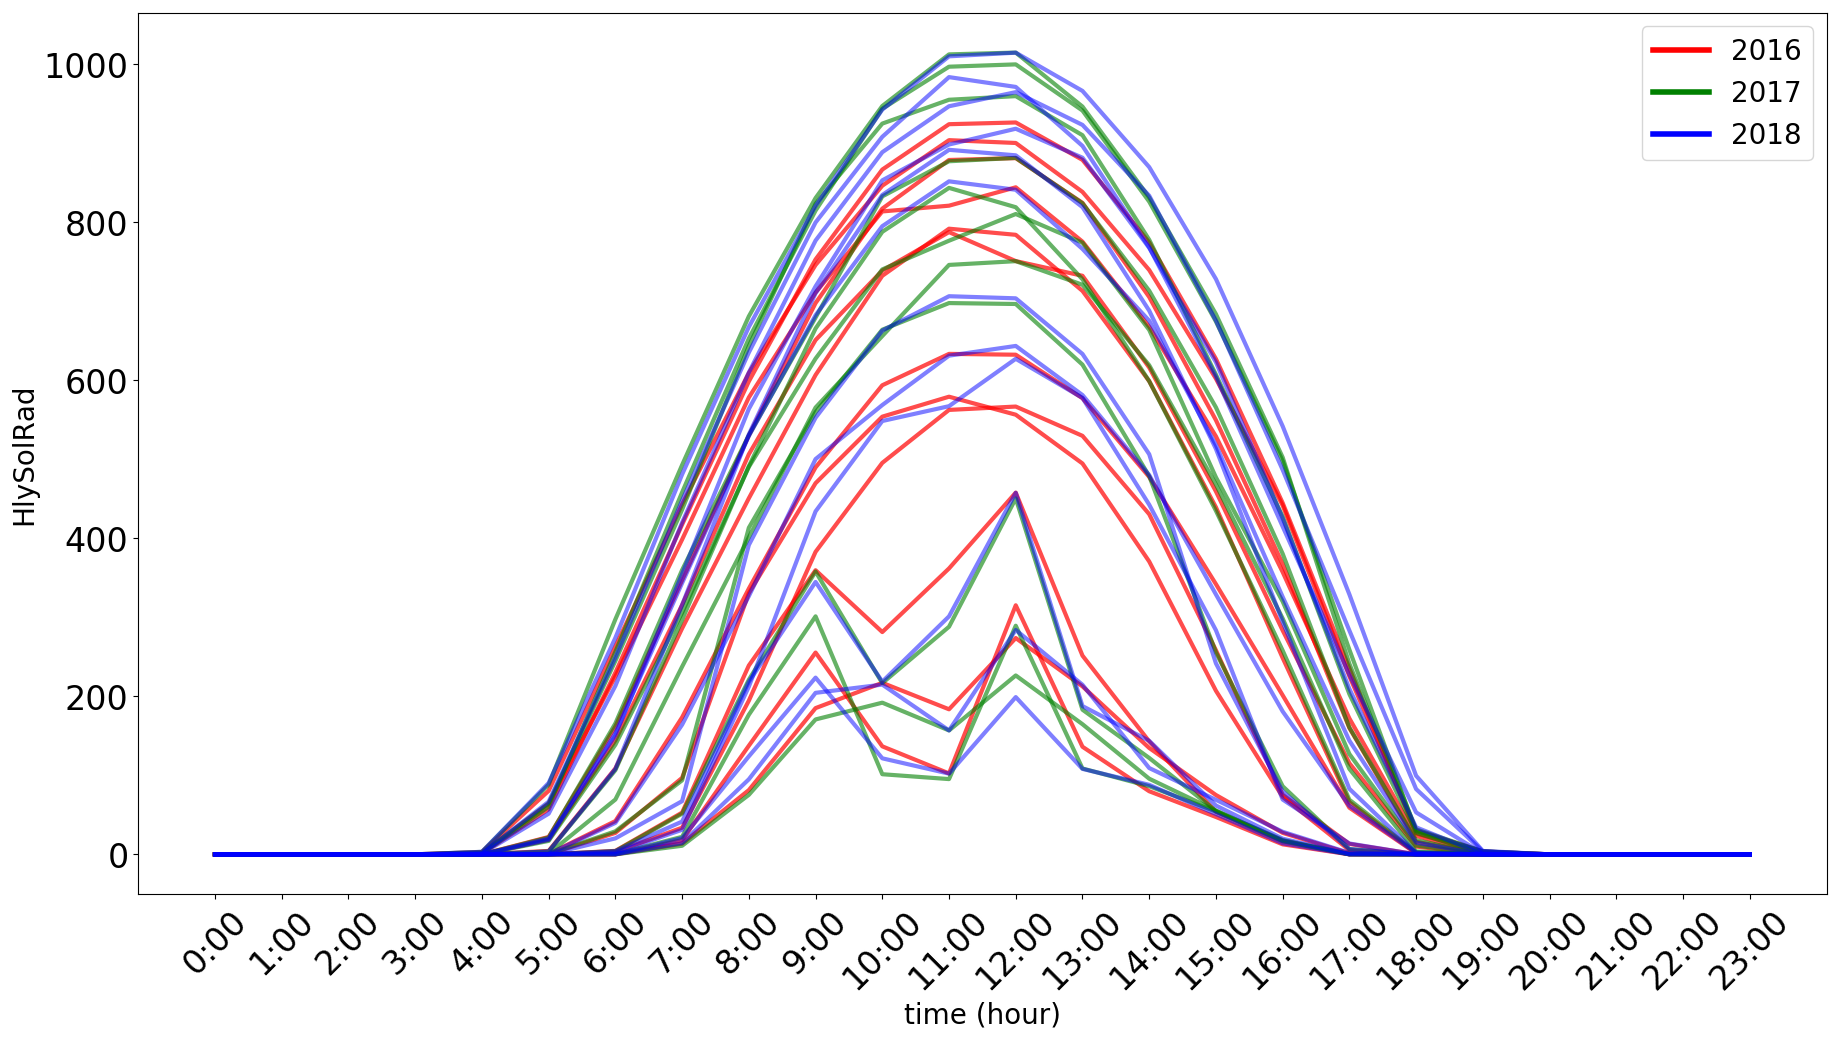
\includegraphics[width=0.9\textwidth]{images/3year7solar.png}
	\caption{36-month Solar Graph for Station 7}\label{fig:solar}
\end{figure}
\end{frame}

\begin{frame}
	In Fig.~\ref{fig:202multi} we can see a similar issue as we saw in Fig.~\ref{fig:7multi}. Knowing which stations have inaccurate data for certain time period could help future predictive model when we know what data we can trust.
\end{frame}

\begin{frame}
\frametitle{36-month Graph for Station 202}
\centering
\begin{figure}
	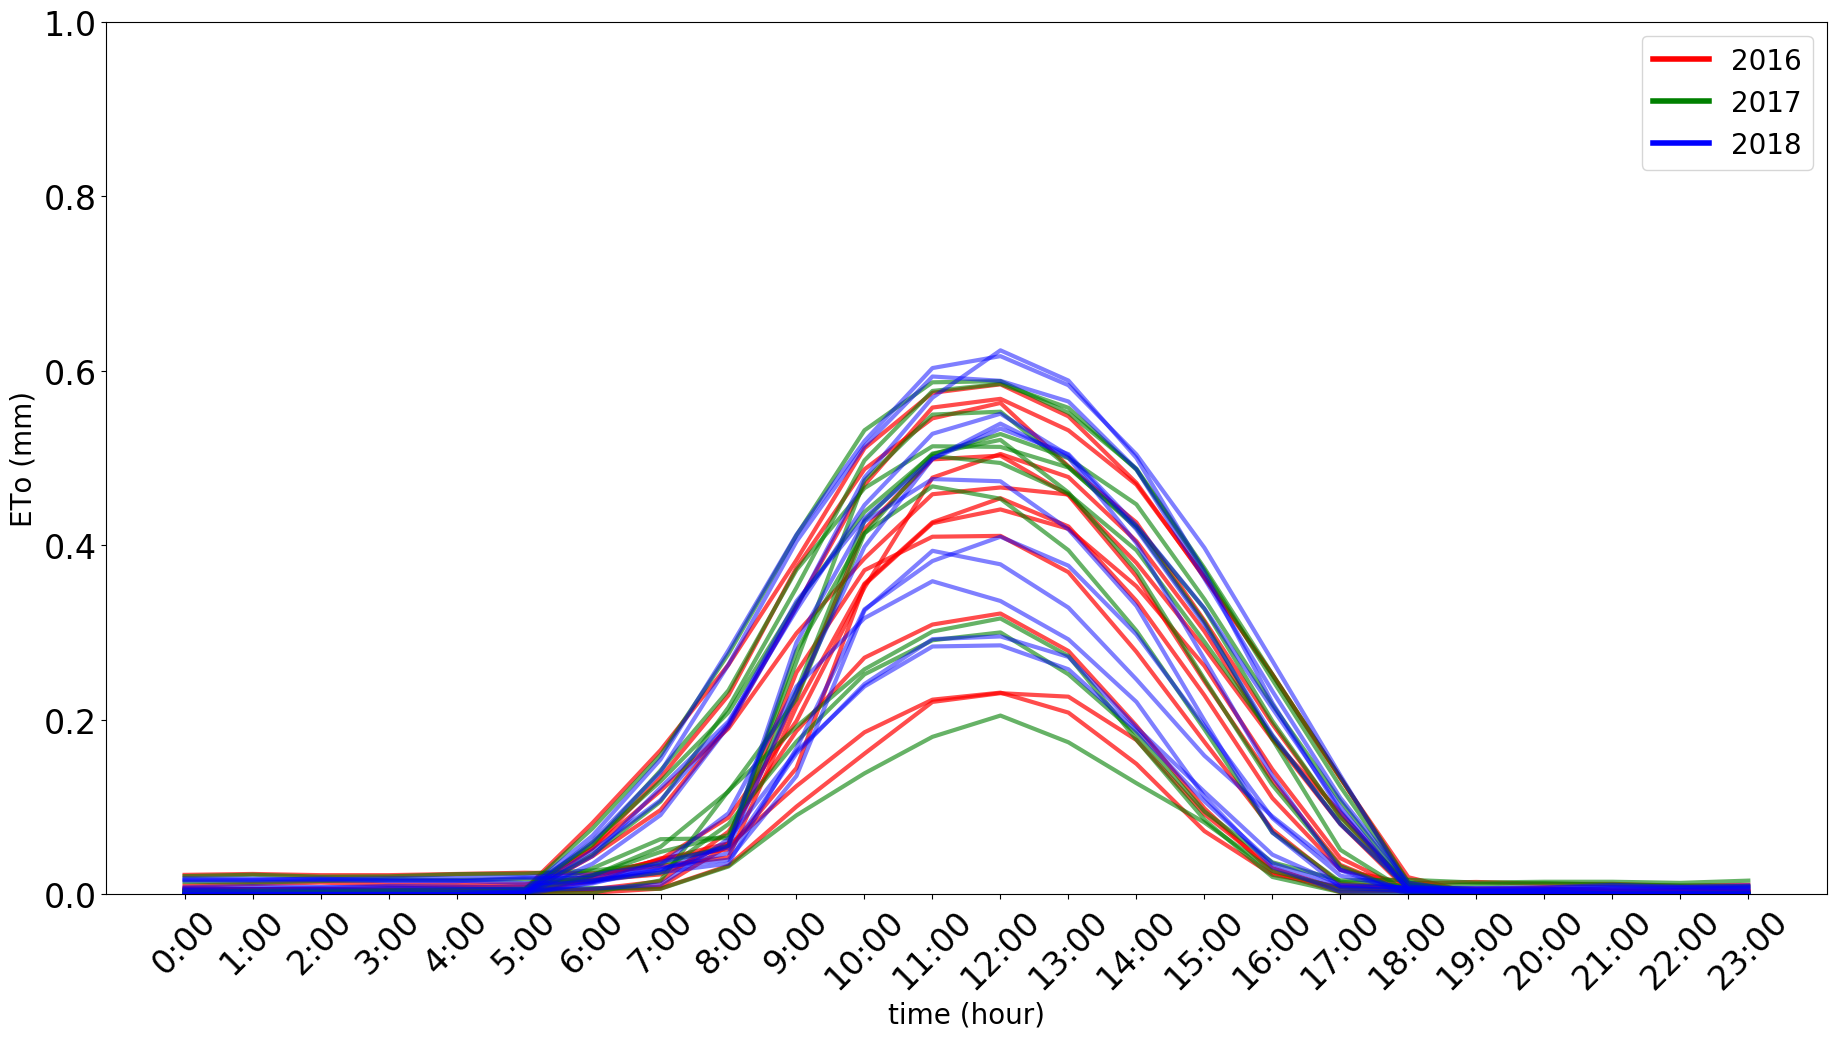
\includegraphics[width=0.9\textwidth]{images/202multi.png}
	\caption{36-month Graph for Station 202}\label{fig:202multi}
\end{figure}
\end{frame}


\section{Questions}
\begin{frame}
	\begin{center}
		{\fontsize{20}{20}\selectfont
			\textbf{Questions?}
		}
	\end{center}
\end{frame}


\end{document}
